% !TeX spellcheck = en_US 

\chapter{Background}

\section{Data Management Layer} \label{chap:DML}
A Distributed Test Support System consists of multiple independent computer systems called nodes. A node may have hardware interfaces to communicate with different bus systems. Additionally, processes called \ac{pu} are executed on a node to process data from the hardware interfaces or to generate data for transmission. The nodes collaborate in a common test environment, therefore it is necessary to exchange data between them. The exchange of data between hardware interfaces and Processing Units, including the exchange between different nodes is facilitated by the \ac{dml}.

This chapter provides an overview of the DML and explains the process of sending and receiving data according to \cite{dml01}.

\subsection{Fundamentals}
\ac{dml} uses a publish-subscribe model to exchange data with the Processing Units. This enables the Processing Units to receive only the required messages from the interfaces. This principle is implemented through the use of a 64-bit identifier called a \ac{dml} ID. Each message has a unique \ac{dml} ID.  The structure of the \ac{dml} ID is shown in Figure \ref{fig:DmlId}.

\begin{figure}[h!]
    \centering
    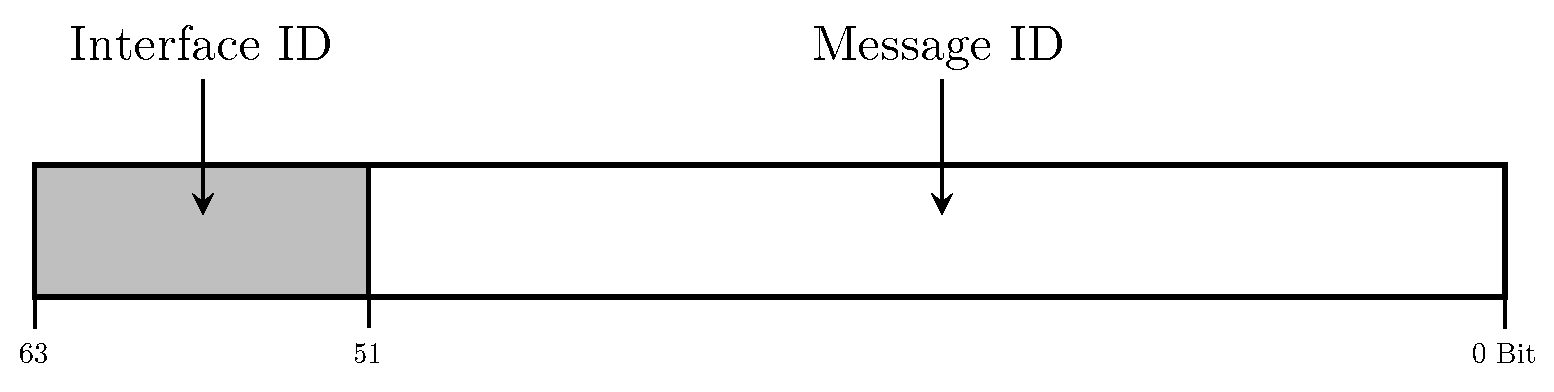
\includegraphics[width=0.8\linewidth]{figures/dml/dml01.pdf}
    \caption[Structure of the DML ID]{Structure of the \ac{dml} ID. Adapted from: \cite{dml01}.}
    \label{fig:DmlId}
\end{figure}

The \ac{dml} ID consists a 12-bit \textit{Interface ID} assigned to each interface by the Test Support System. In addition, a 52-bit \textit{Message ID} is part of the \ac{dml} ID. This contains fields for the unique identification of a message, depending on the bus system implemented at the respective hardware interface.

The current implementation connects the involved independent computer systems using a \ac{pcie}-based solution called Dolphin Interconnect \cite{add01, dml01}. This connection is the focus of this thesis since an Ethernet network based on \ac{udp} is to be investigated as a possible, more cost-efficient, alternative.

\ac{dma} is primarily used as a method of communication between all components involved. It is described in chapter \ref{chap:hwdependcode}.

\subsection{Receive Path}

\subsubsection{Single Node Operation}
This section outlines the procedure for receiving data when a subscribing Processing Unit is present on the local node.

When a message is received by a hardware interface (see Figure \ref{fig:DmlRecSingleNode}, Arrow 1), the interface uses \ac{dma} to copy the data to a \ac{fifo} buffer (see Figure \ref{fig:DmlRecSingleNode}, Arrow 2). A \ac{fifo} buffer is implemented as a ring buffer and is located in the main memory of the node. Each interface has a separate \ac{fifo} buffer, which allows for asynchronous access without mutual exclusion, as the payload and metadata of the \ac{fifo} buffer is only written to by a single entity. Additionally, the it is only accessed by one reader, the Data Manager.

The Data Manager, a process running on each node, polls all of the \ac{fifo} buffers of the node at a specified time interval. If a new message is found in a \ac{fifo} and there is a subscriber for that message, it is processed further.

If a subscriber exists on the local node, referred to as Single Node Operation, the Data Manager copies the message to the monitor memory (see Figure \ref{fig:DmlRecSingleNode}, Arrow 3). From there, it can be read by the subscribing Processing Units. \\

\begin{figure}[h!]
    \centering
    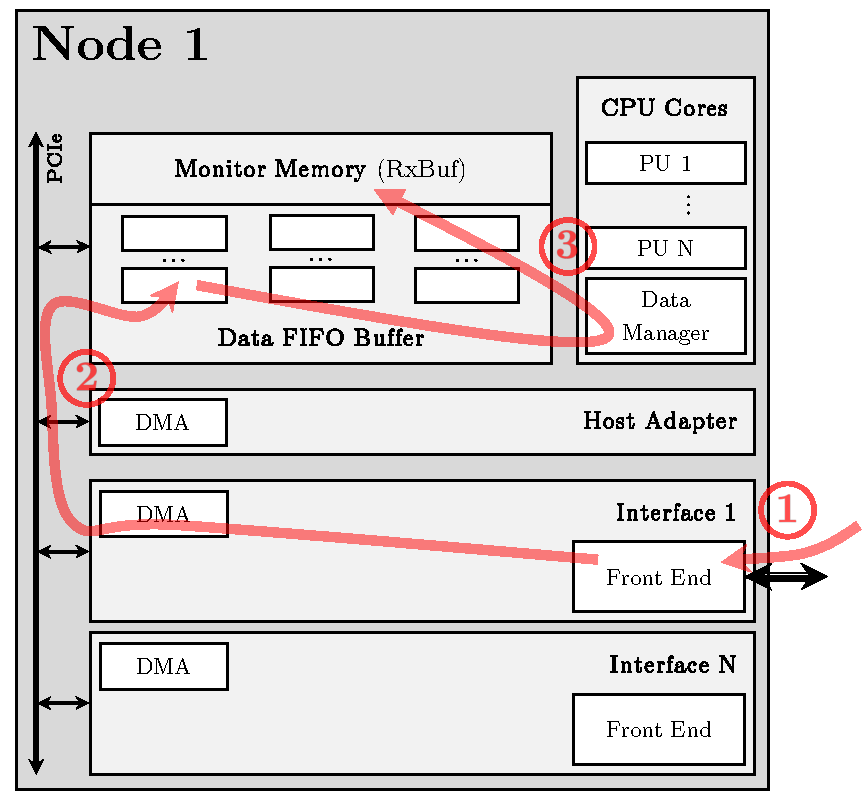
\includegraphics[width=0.48\linewidth]{figures/dml/dml02a.pdf}
    \caption[DML Receive Path in Single Node Operation]{\ac{dml} Receive Path in Single Node Operation. Adapted from: \cite{dml01}.}
    \label{fig:DmlRecSingleNode}
\end{figure}

\subsubsection{Multi Node Operation}
This section covers the procedure for receiving data when a subscribing Processing Unit is present on a remote node of the Distributed Test Support System. The process depicted in Figure \ref{fig:DmlRecMultiNode} for receiving a message (Arrow 1) and copying it to the \ac{fifo} buffer (Arrow 2) does not differ from the single node operation.

If a subscriber for a message exists on a remote node, the message must be forwarded by the Data Manager. To achieve this, the nodes exchange subscriber lists. This forwarding process is illustrated in Figure \ref{fig:DmlRecMultiNode}, Arrow 3. The Data Manager of the local node copies the message by \ac{dma} over the Dolphin Interconnect into a \ac{fifo} buffer of the remote node. Each node has, in addition to the \ac{fifo} buffers for each interface of the node, a \ac{fifo} buffer for each remote node in the Distributed Test Support System.

The Data Manager of the remote node then copies the message to the monitor memory (see Figure \ref{fig:DmlRecMultiNode}, Arrow 4), similar to the local distribution. \\

\begin{figure}[h!]
    \centering
    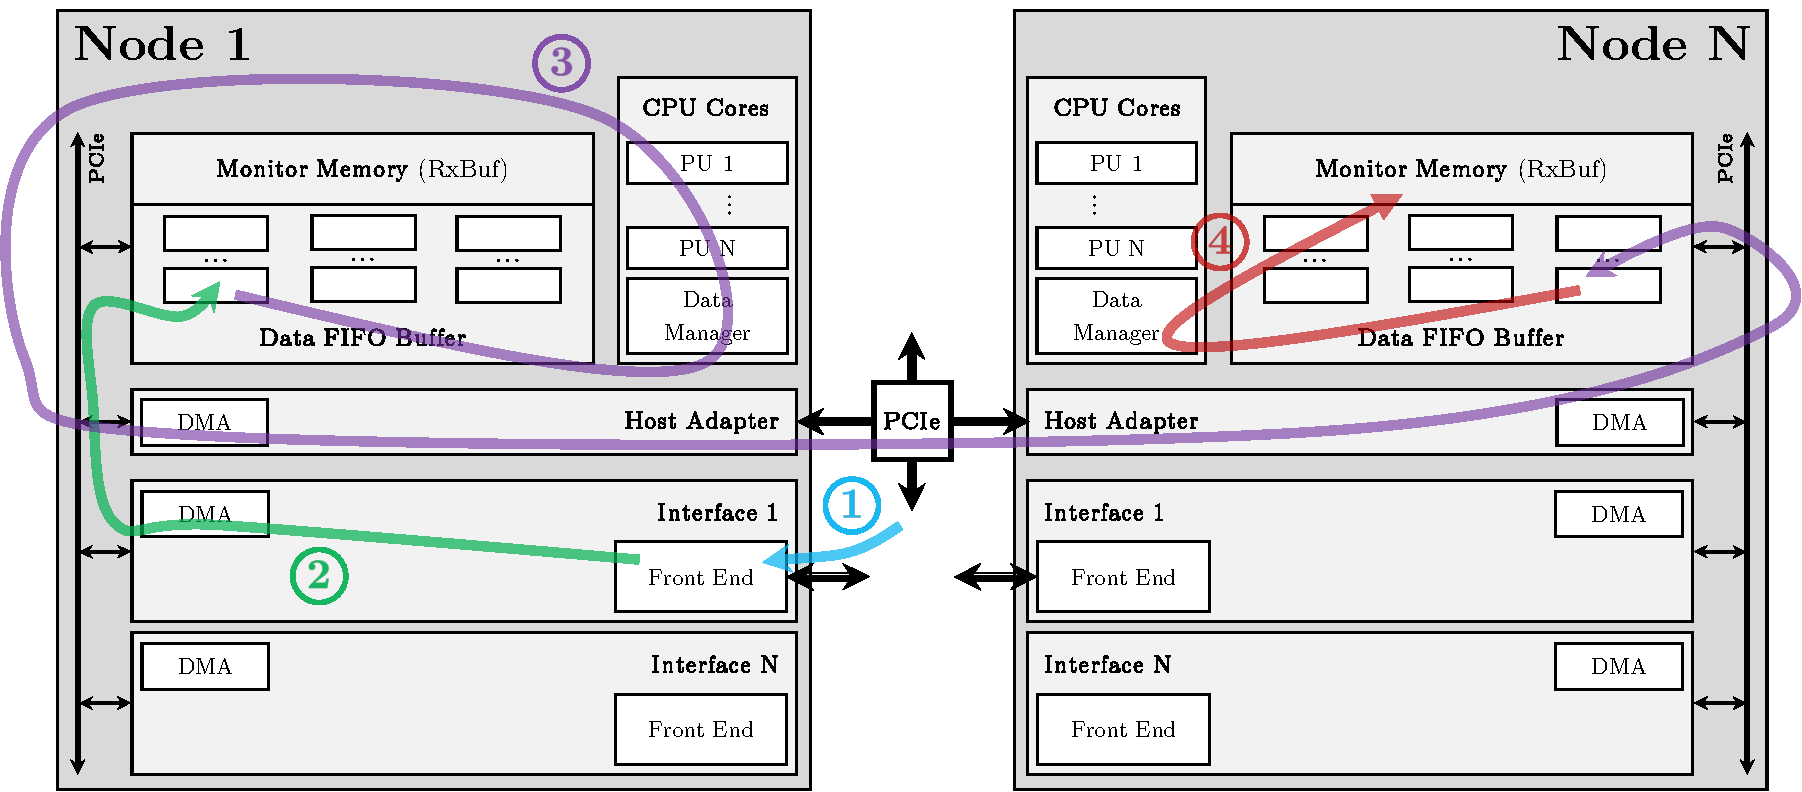
\includegraphics[width=\linewidth]{figures/dml/dml02b.pdf}
    \caption[DML Receive Path in Multi Node Operation]{\ac{dml} Receive Path in Multi Node Operation. Adapted from: \cite{dml01}.}
    \label{fig:DmlRecMultiNode}
\end{figure}



\subsection{Transmit Path}

\subsubsection{Single Node Operation}
This section outlines the procedure for sending data when the interface is located in the same node as the Processing Unit that intends to send it.

To send a message on a bus system using a hardware interface, a Processing Unit writes the message into a \ac{fifo} buffer (see figure \ref{fig:DmlTransSingleNode}, Arrow 1). It is important to note that these \ac{fifo} buffers are distinct from those on the receiving side. Each node in the Distributed Test Support System has a \ac{fifo} for every processing unit and for every other remote node.

The Data Manager also polls these \ac{fifo} buffers. If the message is intended for an interface on the same node, the Data Manager copies it into the Transmit \ac{fifo} (Tx \ac{fifo}) of that interface (see Figure \ref{fig:DmlTransSingleNode}, Arrow 2). The interface then copies the message that will be sent out next on the bus system into the Tx Buffer (see Figure \ref{fig:DmlTransSingleNode}, Arrow 3). A composer mechanism is used to reuse certain parts of a previous message, which allows a Processing Unit to send only the parts that have changed from the prior message. The composer then builds the complete message based on this information. It is then transmitted through the front end of interface in accordance with the timing of the corresponding bus system. \\

\begin{figure}[!htbp]
    \centering
    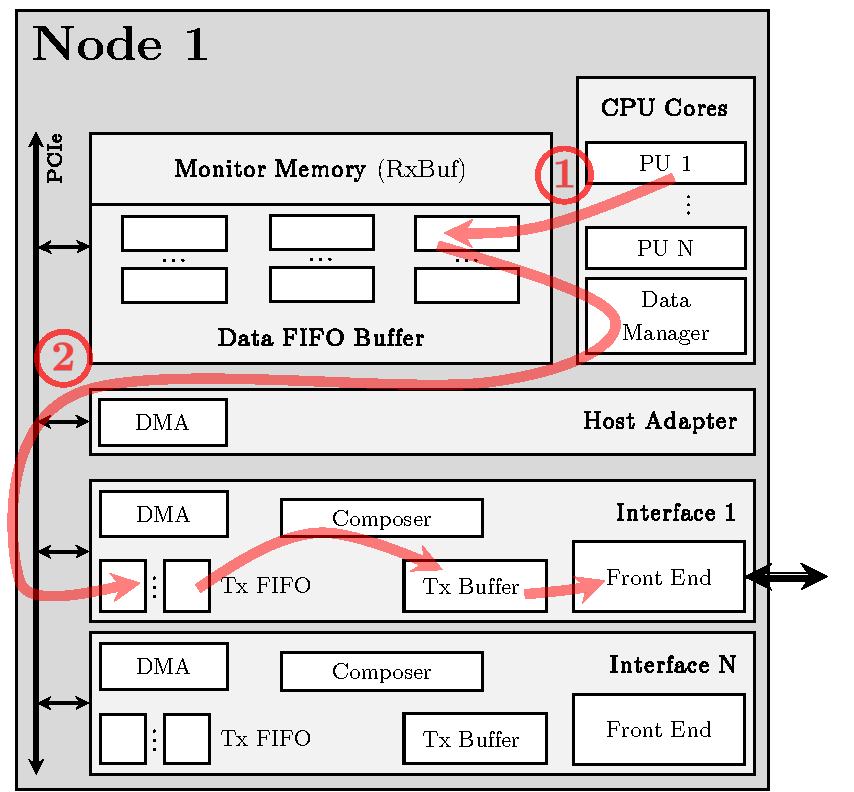
\includegraphics[width=0.48\linewidth]{figures/dml/dml03a.pdf}
    \caption[DML Transmit Path in Single Node Operation]{\ac{dml} Transmit Path in Single Node Operation. Adapted from: \cite{dml01}.}
    \label{fig:DmlTransSingleNode}
\end{figure}


\subsubsection{Multi Node Operation}
This section describes the procedure when a Processing Unit wants to send data over an interface located on a remote node. Similar to the Single Mode Operation, the Processing Unit writes the message to a \ac{fifo} buffer (see Figure \ref{fig:DmlTransMultiNode}, Arrow 1), which is polled by the data manager.

If the message is intended for an interface of a remote node, the Data Manager of the local node copies it using \ac{dma} over the Dolphin Interconnect to its \ac{fifo} buffer on the remote node (see Figure \ref{fig:DmlTransMultiNode}, Arrow 2). The Data Manager of the remote node then places it in the Tx \ac{fifo} of the corresponding interface (see Figure \ref{fig:DmlTransMultiNode}, Arrow 3), from where it is, if required, processed the composer and copied to the Tx Buffer (see Figure \ref{fig:DmlTransMultiNode}, Arrow 4). Subsequently, the message is transmitted through the front end of the interface. \\

\begin{figure}[!h]
    \centering
    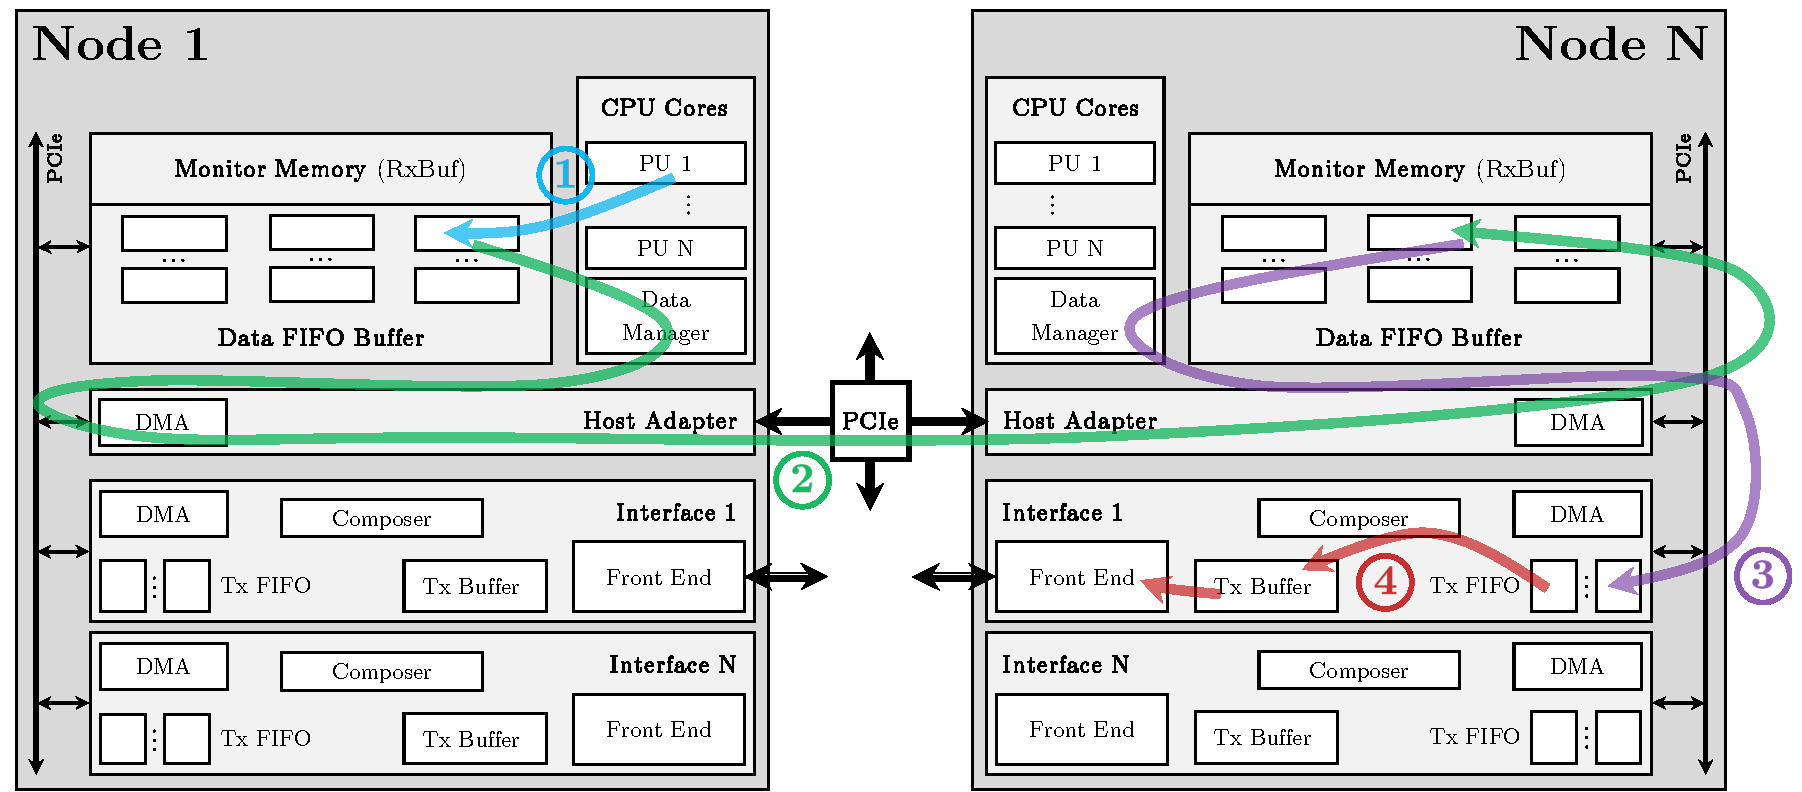
\includegraphics[width=\linewidth]{figures/dml/dml03b.pdf}
    \caption[DML Transmit Path in Multi Node Operation]{\ac{dml} Tranismit Path in Multi Node Operation. Adapted from: \cite{dml01}.}
    \label{fig:DmlTransMultiNode}
\end{figure}

\clearpage


\section{TCP/IP Reference Model} \label{chap:RefModel}

Protocols are the basis for communication between instances in a network. They specify rules that must be followed by all communication partners \cite{Tanenbaum2010}. Reference models arrange protocols hierarchically in layers. Each layer solves a specific part of the communication task and uses the services of the layer below while providing certain services to the layer above \cite{Weigel2021}.

\begin{figure}[h]
    \centering
    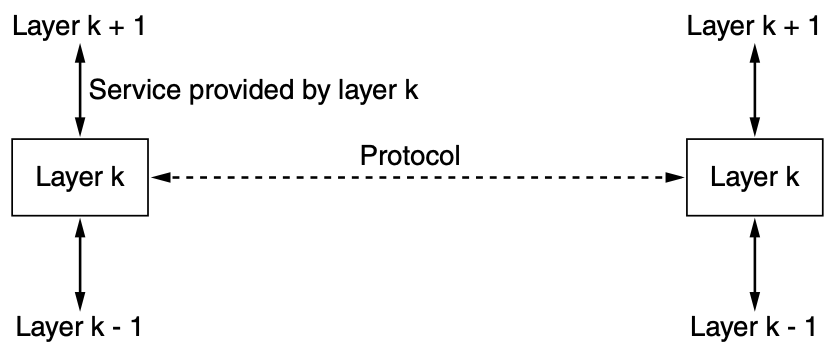
\includegraphics[width=0.7\linewidth]{figures/tcpip_refmodel/image1.png}
    \caption[Relationship between Service and Protocol]{Relationship between Service and Protocol. Source: \cite{Tanenbaum2010}.}
    \label{fig:ServiceProtRelation}
\end{figure}

Figure \ref{fig:ServiceProtRelation} illustrates the relationship between service and protocol. A service refers to a set of operations that a layer provides to the layer above it, and it defines the interface between the two layers \cite{Tanenbaum2010}.

A protocol is a set of rules that define the format of messages exchanged within a layer \cite{Tanenbaum2010}. These rules define the implementation of the service offered by the layer The transparency principle applies, meaning that the implementing protocol is transparent to the service user and can be changed as long as the service offered remains unchanged \cite{Weigel2021}.

\begin{figure}[h!]
    \centering
    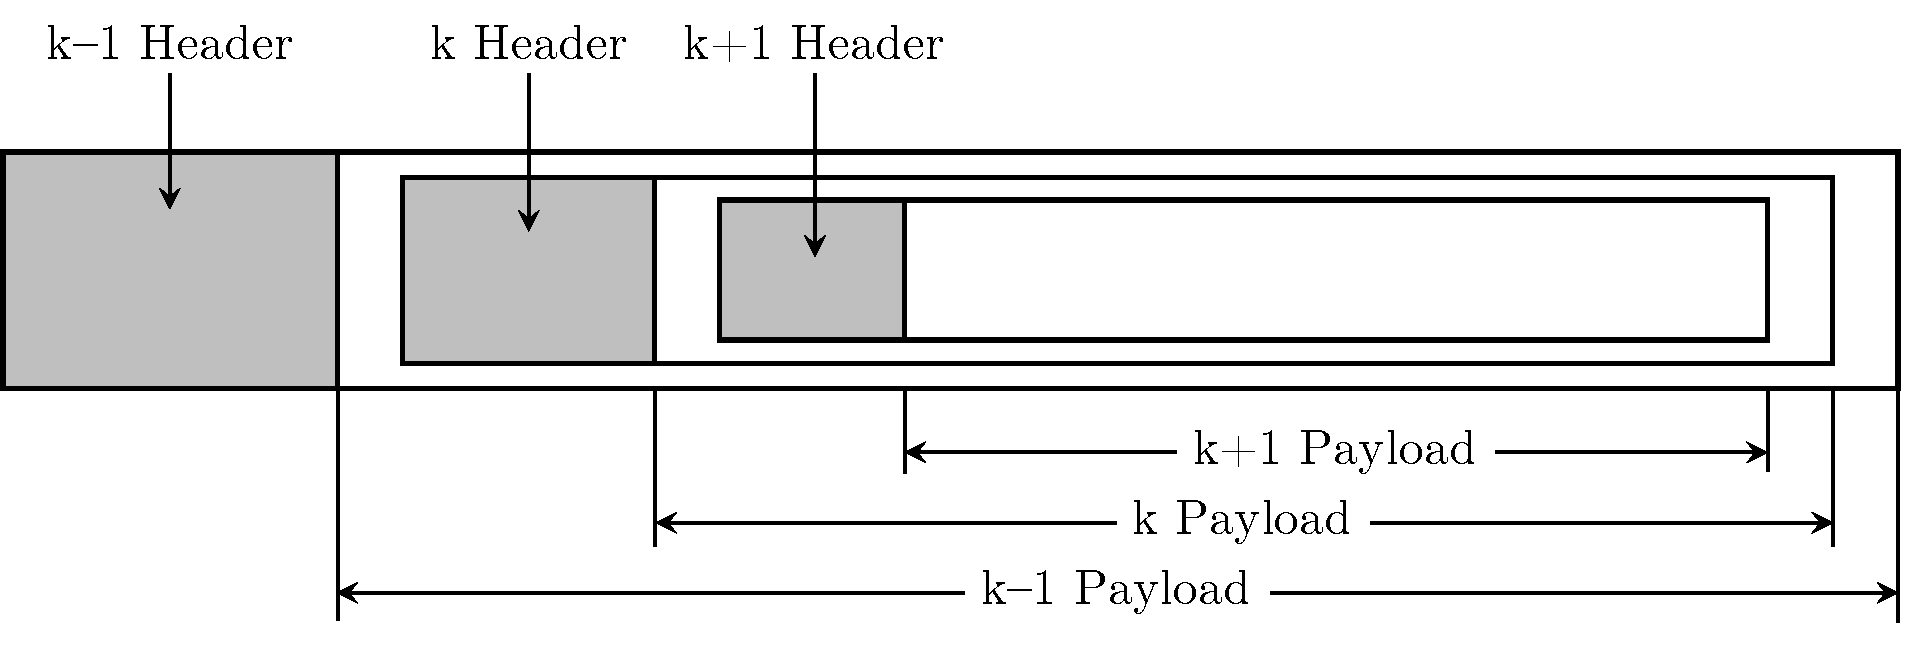
\includegraphics[width=1\linewidth]{figures/tcpip_refmodel/image2.pdf}
    \caption[Encapsulation Principle]{Encapsulation Principle. Adapted from: \cite{Tanenbaum2010}.}
    \label{fig:EncapsulationPrinciple}
\end{figure}

Protocols define the format of control information required by layer k to provide the service. This information is attached as a header or trailer to the data of layer k + 1, known as the payload, and is removed by the receiving instance. This principle is known as the `Encapsulation Principle' and is illustrated in Figure \ref{fig:EncapsulationPrinciple} \cite{Tanenbaum2010}.



\subsection{Introduction of the Reference Model}

The following section presents a explanation of the TCP/IP reference model. Compared to the \ac{osi} reference model, it is a more pragmatic framework that focuses on Internet functionality, compared to the comprehensive seven-layer scheme for network architecture of \ac{osi}. Throughout this section, it will be refered to the hybrid reference model proposed by Andrew S. Tanenbaum in \cite{Tanenbaum2010}. Figure \ref{fig:RefModel} shows this hybrid reference model. The physical layer is at the bottom, and the application layer is at the top. The tasks of each layer are briefly described here. For additional information, please refer to \cite{Tanenbaum2010}.

\begin{figure}[h]
    \centering
    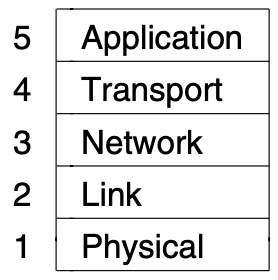
\includegraphics[width=0.25\linewidth]{figures/tcpip_refmodel/image3.png}
    \caption[Hybrid TCP/IP Reference Model]{Hybrid TCP/IP Reference Model. Source: \cite{Tanenbaum2010}.}
    \label{fig:RefModel}
\end{figure}
	
	
\begin{itemize}
\item The \textbf{Physical Layer} serves as the interface between a network node and the transmission medium, responsible for transmitting a bit stream. This involves line coding, which converts binary data into a signal. Additionally, the physical layer encompasses the transmission medium and the connection to this medium \cite{Tanenbaum2010, Weigel2021}.
\item The \textbf{Link Layer} facilitates reliable transmission of a sequence of bits (called a frame) between adjacent network nodes. This encompasses frame synchronization, which involves detecting frame boundaries in the bit stream, error protection, flow control, channel access control, and addressing \cite{Weigel2021}.
\item The \textbf{Network Layer} provides end-to-end communication between two network nodes. This includes addressing and routing \cite{Tanenbaum2010, Weigel2021}.
\item The \textbf{Transport Layer} provides the transfer of a data stream of any length between two application processes. This involves collecting outgoing messages from all application processes and distributing incoming messages to them \cite{Weigel2021}.
\item The \textbf{Application Layer} serves as the interface to the application. It is responsible for implementing protocols for network use, such as file transfer or network management \cite{Weigel2021}.
\end{itemize}



\subsection{Protocols of the Reference Model} \label{chap:ProtosRefModel}

\begin{figure}[h]
    \centering
    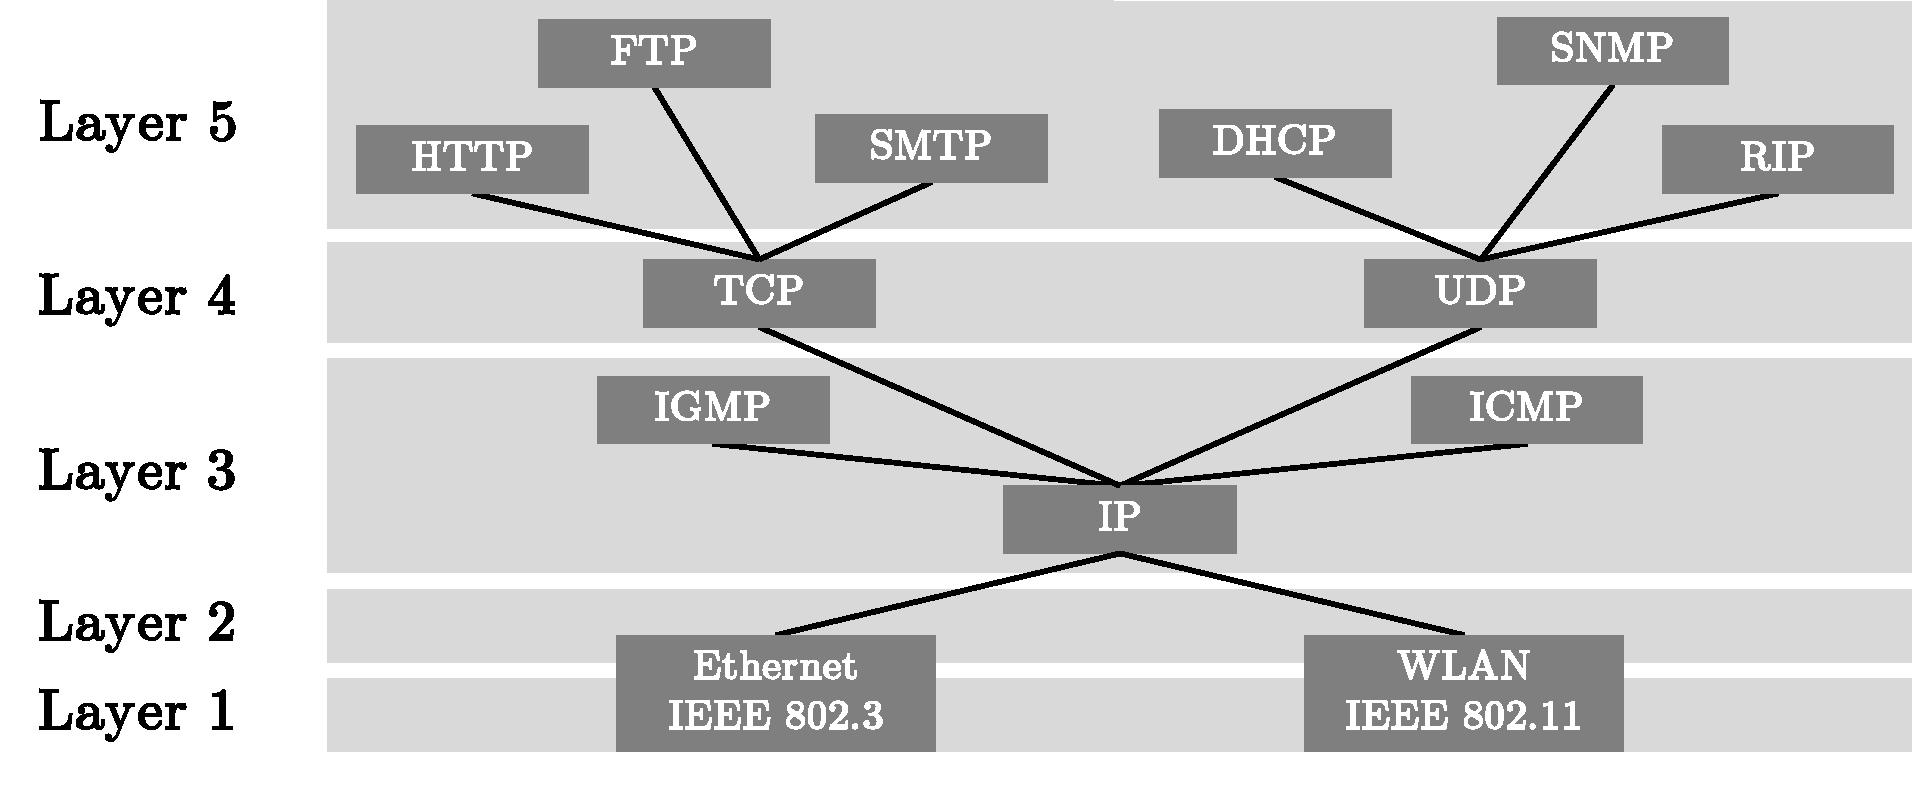
\includegraphics[width=1\linewidth]{figures/tcpip_refmodel/image4.pdf}
    \caption[Selection of important Protocols of the hybrid TCP/IP Reference Model]{Selection of important Protocols of the hybrid TCP/IP Reference Model. Adapted from: \cite{Weigel2021}.}
    \label{fig:RefModelProtos}
\end{figure}

Figure \ref{fig:RefModelProtos} shows a selection of important protocols of the TCP/IP reference model including their assignment to the respective layer. The illustration also shows the dependency of the protocols on each other.

In this section, the characteristics of the protocols \acs{tcp}, \acs{udp}, \acs{ip} and Ethernet (\acs{ieee} 802.3), which are relevant for this work, are explained in detail according to \cite{Tanenbaum2010}. Further information about the protocols of the TCP/IP reference model can be found in \cite{Tanenbaum2010}.


\subsubsection{Ethernet (IEEE 802.3)}
Ethernet, as defined by \ac{ieee} standard 802.3, specifies both hardware and software for wired data networks.  This means that Ethernet includes both the physical layer and the link layer of the presented hybrid TCP/IP reference model.


\paragraph{Ethernet Physical Layer}
The Ethernet physical layer consists of a number of standards that define different media types associated with different transmission rates and cable lengths. 

Ethernet defines physical layer standards with transmission rates ranging from 10 Mbit/s to 1.6 Tbit/s, which is currently under development as the 802.3dj standard \cite{IEEEOpeningPlenary}. Both fiber and copper are used as transmission media. In the following, the 802.3an standard will be briefly discussed, since it is the one that will be used most in this thesis.

The 802.3an standard was published in 2006 and defines data transmission with a transmission rate of 10 Gbit/s over twisted-pair cables \cite{10GigabitEthernet}, also referred to as 10 GbE. Twisted-pair cables are copper cables in which pairs of copper wires are twisted together to reduce electromagnetic interference. Twisted-pair cables are divided into categories based on various characteristics, such as shielding or twist strength \cite{isoiec11801}. For 802.3an, a maximum cable length of 100 meters is specified in conjunction with Cat7 cables. Also, the RJ45 connector is specified as the plug connector.

According to 802.3an, the PAM16 line coding is used for Ethernet at 10 Gbit/s. It uses the principle of pulse amplitude modulation, which is described in detail in \cite{PulseAmplitudeModulation}. PAM16 allows the transmission of data by varying the amplitude of a signal in 16 different stages. Each stage represents four bits of information.

In addition to 802.3an, the Ethernet physical layer according to 802.3ae was also used in this work. This also defines the physical layer with a transmission rate of 10 Gbit/s. However, fiber optic cables are used in conjunction with transceiver modules called \ac{sfp} \cite{10GigabitEthernet}.

\paragraph{Ethernet Link Layer} \label{chap:EthLinkLayer}
At the link layer, Ethernet defines frame formatting, addressing, error detection, and access control. This is also called the \ac{mac} sublayer.

\begin{figure}[h]
    \centering
    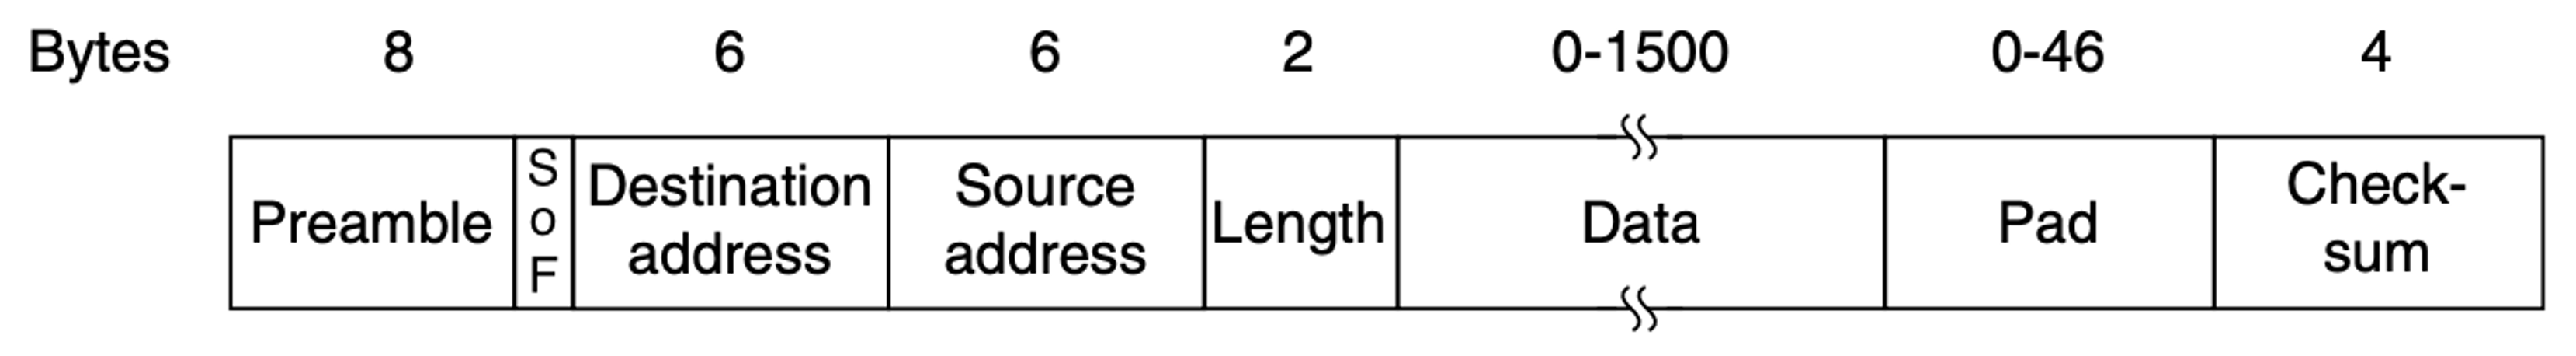
\includegraphics[width=1\linewidth]{figures/tcpip_refmodel/image5.png}
    \caption[Structure of the Ethernet frame]{Structure of the Ethernet frame. Source: \cite{Tanenbaum2010}.}
    \label{fig:EthernetFrame}
\end{figure}

Figure \ref{fig:EthernetFrame} shows the \ac{ieee} 802.3 frame format. The Ethernet header consists of the fields '\textit{Destination address}', '\textit{Source address}' and '\textit{Length}' and therefore has a size of 14 bytes.

Each frame begins with a \textit{preamble}. This has a length of 8 bytes and contains the bit sequence 10101010. An exception is the last byte, which contains the bit sequence 10101011 and is referred to as the \textit{Start of Frame} (SoF). The preamble is used for synchronization between the sender and receiver. The last byte of the preamble marks the start of a frame \cite{Tanenbaum2010}.

This is followed by the \textit{destination} and \textit{source address}. This is the \ac{mac} address, which is uniquely assigned globally to a network interface \cite{Weigel2021}. This consists of a manufacturer code with a length of 3 bytes, followed by the serial number of the network interface, which also has a length of 3 bytes. The \ac{mac} address enables the Ethernet protocol to uniquely identify a station in the local network.

The \textit{Length} field specifies the length of the data field. In \ac{ieee} 802.3 Ethernet, this has a maximum length, called the \ac{mtu}, of 1500 bytes. However, there are Ethernet implementations that use a larger \ac{mtu} than specified in the original standard. These are known as jumbo frames \cite{EthernetJumboFrames2009}. Jumbo frames can increase network throughput and reduce the utilization of the \ac{CPU}, as demonstrated in studies \cite{swsetup03}. It is important to ensure that all network participants support jumbo frames to avoid packet loss \cite{swsetup04}.

In addition to a maximum length, the Ethernet standard also specifies a minimum length. An entire Ethernet frame must therefore have a minimum length of 64 bytes from the destination address to the checksum. To ensure that this can be achieved even with a small data field, padding information is added. The specification of the minimum length is related to the access control used.

The Ethernet frame ends with a 4-byte \textit{checksum} that is used for the \ac{crc} based on polynomial divisions, as explained in \cite{Tanenbaum2010}.  This checksum serves to detect errors during transmission.

Ethernet originally used a shared transmission medium, allowing multiple communication participants to use it simultaneously. To control access, the \ac{mac} sublayer employs the \ac{csmacd} algorithm, ensuring that only one device transmits data at a time. Each device listens to the medium (carrier sense) before sending data to determine whether it is free. It also performs collision detection to determine whether two devices have started sending at the same time. In such a case, the devices stop the transmission and retry it after a random waiting time to avoid the collision \cite{Tanenbaum2010}.

The 802.3an specification for 10 Gigabit Ethernet is exclusively for point-to-point full-duplex connections, which eliminates the need for access control such as \ac{csmacd}. As a result, it is no longer included in the specification \cite{10GbEDefinition}.

In order to connect multiple network devices with point-to-point connections, Ethernet switches are used. They have multiple ports and forward packets based on the MAC address. Ethernet switches operate on layer 2 of the reference model.

To summarise, with Ethernet there is no guarantee that data will be transmitted reliably and without loss. Although Ethernet uses \ac{crc} for error detection, faulty frames are generally discarded. Additionally, Ethernet does not provide flow control or overload detection, which must be performed by a higher layer.


\subsubsection{IP}

The \ac{ip} is a central protocol in the TCP/IP reference model. Its tasks include connecting different networks, addressing network participants, and fragmenting packets \cite{Weigel2021}. \ac{ip} is a connectionless protocol that operates on the 'best effort' principle, meaning it does not guarantee delivery.

There are two versions of the Internet Protocol: IPv4 and IPv6. As this work uses the IPv4 protocol, it is presented in more detail below.

\paragraph{IP Header} \label{chap:ipheader}

The IPv4 datagram is divided into a header and a payload. The header typically spans 20 bytes, but may also include an optional variable-length section. The header is shown in Figure \ref{fig:IPHeader}.

\begin{figure}[h]
    \centering
    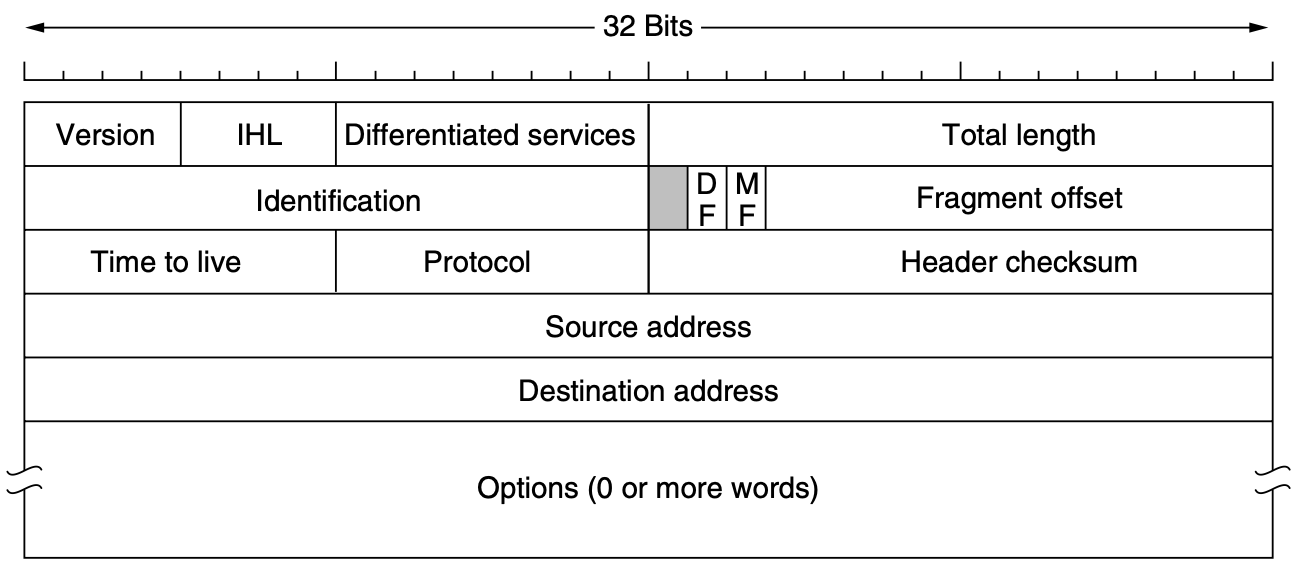
\includegraphics[width=1\linewidth]{figures/tcpip_refmodel/image7.png}
    \caption[Structure of the IP Header]{Structure of the IP Header. Source: \cite{Tanenbaum2010}.}
    \label{fig:IPHeader}
\end{figure}

The first field in the header is the 4-bit \textit{Version} field. This indicates the \ac{ip} version used. For IPv4, the value is always 4.

The \textit{IHL} (Internet Header Length) field specifies the number of 32-bit words in the header. This is necessary because the header can contain options and therefore has a variable length. The minimum value of the field is 5 if there are no options.

The \textit{Differenciated Services} field specifies the service class of a packet, allowing for prioritisation of certain data traffic using \ac{qos}. For a more detailed description of \ac{qos}, please refer to Chapter \ref{background:tuning:qualityofservice}.

The \textit{Total Length} field indicates the total length of the datagram, including the header. Due to the field size of 16 bits, the maximum length is 65535 bytes. However, a packet's length is also limited by the Layer 2 \ac{mtu} \cite{Weigel2021}, resulting in datagrams being split into multiple packets, known as fragmentation. 

The \textit{Identification} field is assigned a number by the sender, which is shared by all fragments of a datagram.

A flag field with a length of 3 bits follows, with the first bit being unused. The second section includes the 'Don't Fragment' (\textit{DF}) flag, which indicates that intermediate stations should not fragment this packet. The third section contains the 'More Fragments' (\textit{MF}) flag, which indicates whether additional fragments follow. This flag is set for all fragments except the last one of a datagram.

The \textit{Fragment Offset} field specifies the position of a fragment in the entire datagram.

The \textit{Time to live} (TTL) field specifies the maximum lifetime of a packet. The TTL value is measured in seconds and can be set to a maximum of 255 seconds. This is done to prevent packets from endlessly circulating in the network.

The \textit{Protocol} field identifies the Layer 4 protocol used for the service. This allows the network layer to forward the packet to the corresponding protocol of the transport layer. The numbering of the protocols is standardized throughout the Internet.

The \textit{Header checksum} field contains the checksum of the fields in the IP header. The IP datagram's user data is not verified for efficiency reasons \cite{Holtkamp2024Internet}. The checksum is calculated by taking the 1's complement of the sum of all 16-bit half-words in the header. It is assumed that the checksum is zero at the start of the calculation for the purpose of this algorithm.

The two 32-bit fields \textit{Source Address} and \textit{Destination Address} contain the Internet Protocol address, called the IP address. Chapter \ref{chap:IPandRouting} provides further details on this topic.

The \textit{Options} field can be used to add additional information to the IP protocol. For example, there are options to mark the route of a packet.


\paragraph{IP Addresses and Routing} \label{chap:IPandRouting}

This section provides a brief description of the structure and important properties of IP addresses. The network examined in this thesis is an isolated local network that is not connected to other networks. As a result, the network layer does not perform any routing based on IP addresses. For further information on routing, please refer to \cite{Tanenbaum2010}.

\begin{figure}[h]
    \centering
    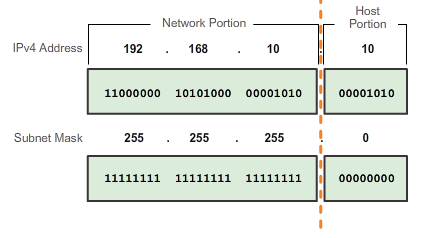
\includegraphics[width=0.8\linewidth]{figures/tcpip_refmodel/image8.png}
    \caption[Structure of the IP address and subnet mask]{Structure of the IP address and subnet mask. Source: \cite{CSE252ImageSubnet}.}
    \label{fig:IPSubnet}
\end{figure}

Every participant on the Internet has a unique address, known as an IP address. This has a total length of 32 bits and a hierarchical structure that divides the IP address into a network portion and a host portion. The division between the two parts is variable and is defined by a so-called subnet mask, which is illustrated in Figure \ref{fig:IPSubnet}. The bits of the network portion of the IP address are marked with ones.

\begin{itemize}
\item The \textbf{network portion} identifies a specific network, such as a local Ethernet network, and is the same for all participants in this network.
\item The \textbf{host portion} identifies a specific device within this network.
\end{itemize}

Routing, which is another important task of the network layer, is based on IP addresses. The packet can be directed to its destination using the network portion of the IP address. The path to the destination is determined by specific routing algorithms. As mentioned earlier, the thesis only considers an isolated local network, so further discussion on routing will be omitted.


\paragraph{Address Resolution Protocol}

The \ac{arp} is an auxiliary protocol of the network layer. Its task is to map the IP addresses to a MAC address and vice versa, as the sending and receiving of data in the underlying link layer is based on these MAC addresses \cite{Weigel2021}.


\paragraph{Fragmentation and Defragmentation} \label{chap:frag}

As explained in \ref{chap:EthLinkLayer}, the link layer defines a maximum data size known as \ac{mtu}. Since IPv4 datagrams have a maximum size of 65535 bytes, they must be divided into smaller packets, or fragments, each with its own IP header.

The IP header (refer to Figure \ref{fig:IPHeader}) contains information necessary for the target system to assemble fragmented packets, a process known as defragmentation. This includes the ID that assigns all fragmented packets to a datagram, as well as the fragment offset that specifies their position within the datagram. The 'More Fragment' flag indicates whether additional fragments will follow.

Fragmentation has the advantage of allowing IPv4 datagrams larger than the \ac{mtu} to be sent, but the disadvantage is that the loss of a single fragment results in the loss of the entire datagram. Additionally, fragmentation can cause packet reordering \cite{IPFragDetail}.

\subsubsection{TCP and UDP}
\ac{tcp} and \ac{udp} are transport layer protocols. As a service, they provide the transmission of a data stream of any length between two application processes. The services of the network layer are used for this purpose.

\paragraph{TCP}

The \acf{tcp} provides \textbf{reliable} transmission of a byte stream in a \textbf{connection-oriented} manner. A virtual connection is established between the two instances before transmission, which is terminated after transmission.

The protocol also implements flow control to ensure reliable data transfer between sender and receiver without losses and to prevent overloading at the receiver. \ac{tcp} provides congestion control to prevent network overload and ensures reliable transmission using Positive Acknowledgement with Re-Transmission (PAR) algorithm \cite{Holtkamp2024Transport}.  

\ac{tcp} is known for its secure data transmission. However, it requires a significant amount of control information to implement its functions. The \ac{tcp} header is 20 bytes in size. In addition to an application identifier (port number), it contains flow control and congestion control information. This overhead can negatively impact transmission speed. Additionally, the data loss from the underlying layers combined with the flow control used by \ac{tcp} leads to delays and reduced throughput, which can have a significant impact on the performance of the application.

\paragraph{UDP}

In contrast to \ac{tcp}, the \acf{udp} is an \textbf{unreliable} and \textbf{connectionless} protocol. The protocol sends packets, called datagrams or segments, individually. \ac{udp} lacks mechanisms for detecting the loss of individual datagrams, and the correct sequence of these is not guaranteed.

\begin{figure}[h]
    \centering
    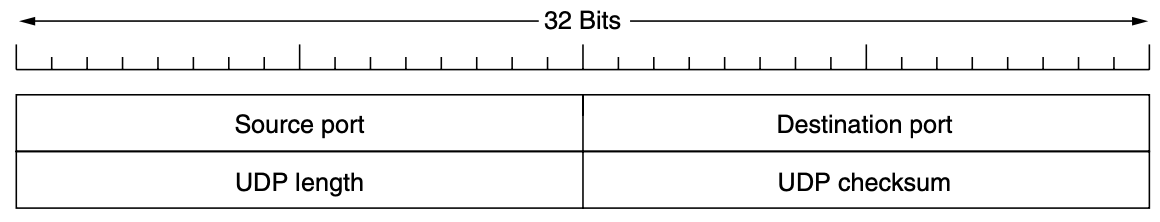
\includegraphics[width=1\linewidth]{figures/tcpip_refmodel/image6.png}
    \caption[Structure of the UDP Header]{Structure of the \ac{udp} Header. Source: \cite{Tanenbaum2010}.}
    \label{fig:UDPHeader}
\end{figure}

Figure \ref{fig:UDPHeader} displays the \ac{udp} header, which has a size of 8 bytes. It is considerably smaller than the TPC header, which has a size of 20 bytes.

The header includes the fields \textit{Source port} and \textit{Destination port} to identify the endpoints in the respective instance. When a packet arrives, the payload is passed to the application using the appropriate port number via the \ac{udp} protocol.

The \textit{\ac{udp} length} field indicates the length of the segment, including the header. The maximum length of data that can be transmitted via \ac{udp} is limited to 65,515 bytes due to the underlying Internet Protocol.

The last field of the header is a 16-bit \textit{\ac{udp} checksum}. This checksum is formed via the so-called IP pseudoheader, which contains the source and destination IP address, the protocol number from the IP header, and the \textit{\ac{udp} length} field of the \ac{udp} header.

Compared to \ac{tcp}, \ac{udp} can achieve higher data transmission speeds due to its lower protocol overhead, as the \ac{udp} header is only 8 bytes in size. Furthermore, \ac{udp} does not require an acknowledgement of the transport or other mechanisms used by \ac{tcp} to provide a reliable connection. This makes it very efficient and reduces processing overhead.

\clearpage

\section{Linux Kernel}
This investigation in this thesis and the Distributed Test Support System use an operating system based on the Linux kernel. Therefore, a brief introduction to this kernel is provided.

The Linux kernel is an operating system kernel that is available under a free software license and has been under development since 1991 \cite{like01}. The Linux kernel is the main component of a Linux operating system and is used by a large number of operating systems, called distributions. Popular examples of such distributions are Ubuntu or Linux Mint, which are used in this thesis.

This chapter will take a closer look at the Linux kernel. However, due to the scope of the Linux kernel, readers are referred to \cite{like02}, \cite{like03} and \cite{like08}, which provide a detailed and comprehensible insight into the Linux kernel. Additionally, a basic knowledge of operating systems is required, which can be obtained from \cite{like05}.

An operating system kernel serves as the interface between the hardware and the processes of a computer system \cite{like04}. It manages hardware resources, schedules processes, and facilitates communication between application software and hardware \cite{like06}.

\begin{figure}[h]
    \centering
    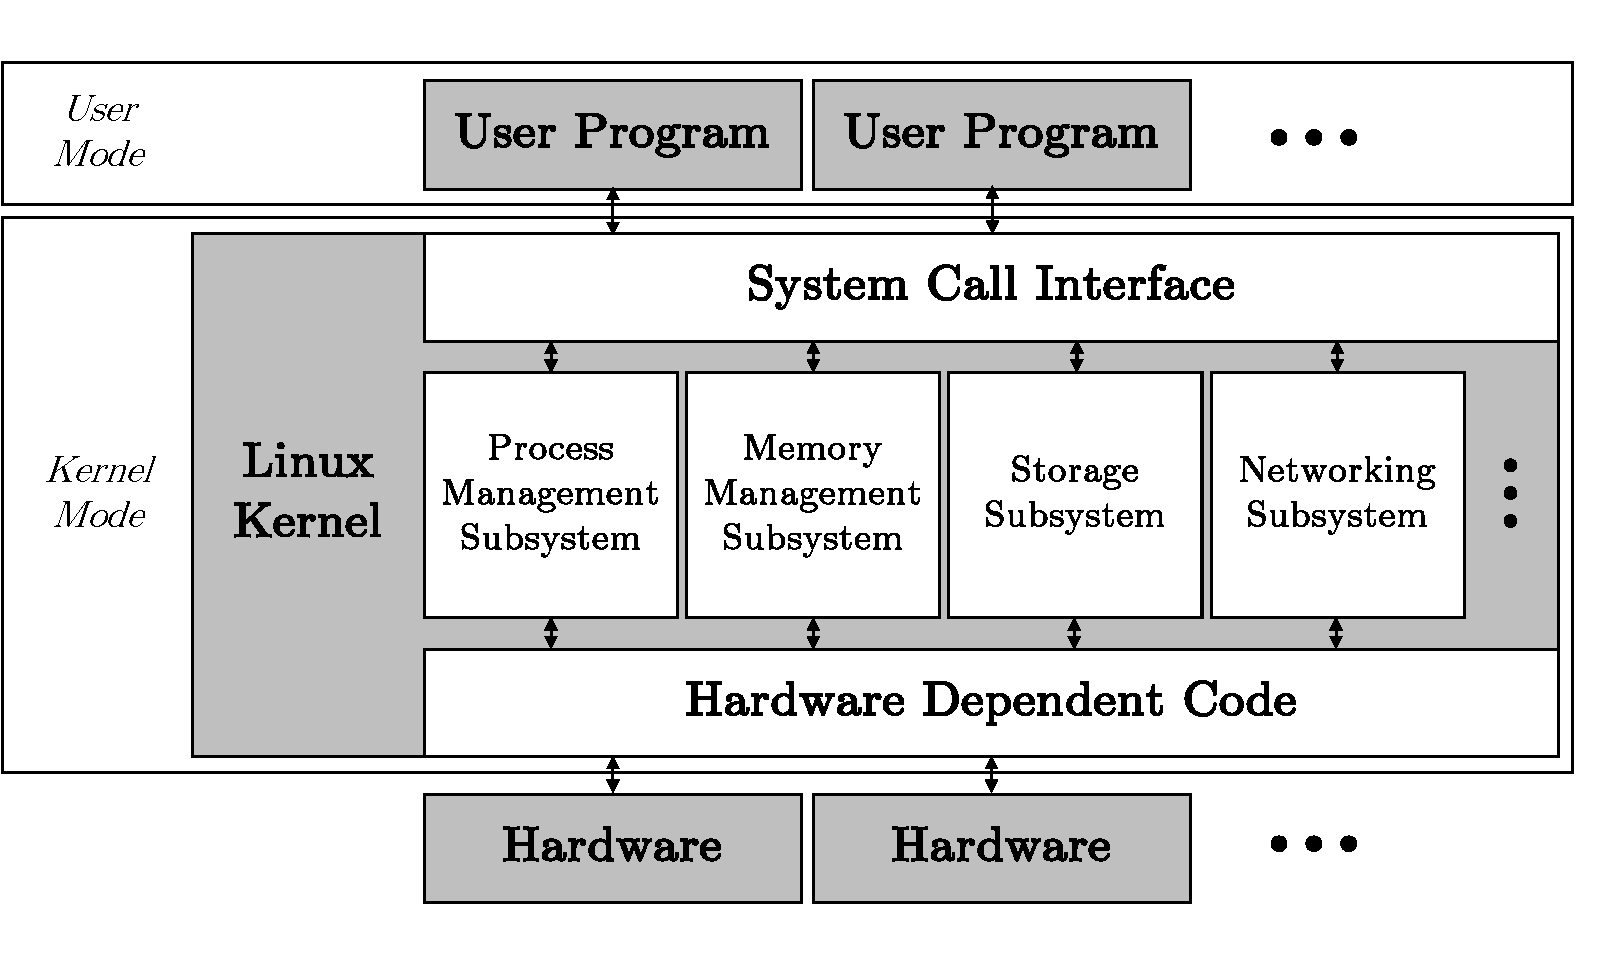
\includegraphics[width=1\linewidth]{figures/linux_kernel/image01.pdf}
    \caption[Simplified Representation of the Linux Kernel with selected Subsystems]{Simplified Representation of the Linux Kernel with selected Subsystems.}
    \label{fig:LinuxKernel}
\end{figure}

Figure \ref{fig:LinuxKernel} presents a condensed overview of the architecture of a Linux operating system. The illustration highlights some selected features of the kernel.

Linux consists of a monolithic kernel. This means that the entire kernel is implemented as a single program, and all kernel services run in a single address space. Communication within the kernel is achieved through function calls \cite{like02}.

This is in contrast to the microkernel, which divides functionalities into separate modules and uses message passing for communication between them. Although the Linux kernel is based on a monolithic approach, it adopts some aspects of a microkernel, such as a modular architecture with different subsystems or the ability to load modules dynamically. However, communication within the kernel occurs through function calls, which provides better performance compared to message passing \cite{like08}.

In the following, the characteristics of the Linux kernel and its environment shown in Figure \ref{fig:LinuxKernel} are described.


\subsection{User Mode and Kernel Mode}

The Linux architecture distinguishes between two basic execution environments: user mode and kernel mode. Application processes run in user mode with restricted rights, while the Linux kernel, which is the main part of the operating system, runs in kernel mode \cite{like02}.

This separation requires corresponding support in the processor. This system monitors aspects such as memory access, branches, or the executed instruction set in user mode and intervenes in the event of unauthorized access, for example, by stopping the process \cite{like06}. The transition between the different execution environments occurs as part of a system call.


\subsection{System Call Interface}

Processes that request a service from the Linux kernel use system calls. These calls are made through a software interrupt (trap), which causes the \ac{CPU} to switch to kernel mode and call the so-called system call handler. In the handler, the requested service is identified using an ID transmitted by the user process, and the corresponding instructions are invoked \cite{like02}. A process or application executes a system call in kernel space. This is also referred to as the kernel running in the context of the process.

In the monolithic kernel, individual instructions call other instructions of the kernel.  This sequence of instructions, executed during a system call, is referred to as the \textit{kernel control path} \cite{like07}.

The Linux kernel is a \textit{reentrant kernel}. Several processes can be executed simultaneously in kernel mode, which also means that the process can be interrupted while instructions are being executed in kernel mode. Functions in a reentrant kernel should therefore only change local variables and not affect global data structures. However, there are also non-reentrant functions in the kernel, for which corresponding locking mechanisms are used \cite{like02}.

It should be noted here that system calls are not the only way to execute instructions in the kernel. According to \cite{like02}, there exist other ways besides system calls:

\begin{itemize}
\item A exception is reported by the \ac{CPU}, which are handled by the kernel for the originating process. An example of this is the execution of an invalid instruction.
\item A peripheral device sends an interrupt signal to the \ac{CPU}, which is processed by a function called the interrupt handler. As peripheral devices work asynchronously to the \ac{CPU}, interrupts occur at unpredictable times.
\item A kernel thread is executed. These run in kernel mode and are mainly used to perform certain tasks periodically.
\end{itemize}


\subsection{Hardware and Hardware Dependent Code} \label{chap:hwdependcode}

As already mentioned, the kernel is the interface between the hardware and the processes of a system. Many operations in the kernel are related to the access of physical hardware.

The Linux kernel distinguishes between three different types of hardware devices [8]:

\begin{itemize}
\item \textbf{Block Devices} – devices with block-oriented addressable data storage (e.g. hard drives)
\item \textbf{Character Devices} – devices that handle data as a stream of characters or bytes (e.g. keyboards)
\item \textbf{Network Devices} – devices that provide access to a network
\end{itemize}

The abstraction layer between the physical hardware and the Linux kernel are device drivers. Their primary function is to initialize the device and register its capabilities with the kernel. Additionally, drivers enable the kernel to access, control, and communicate with the device. Each driver is specific to a device and implements certain predefined interface functions to the Linux kernel, depending on the type of the device. The device drivers are available as modules that can be loaded dynamically at runtime \cite{like09}.

One way for the physical hardware to interact with the kernel via the device drivers is through interrupts, which is referred to as \textit{Interrupt-Driven \ac{io}}. The hardware uses \textit{interrupt requests} to inform about certain events, and the driver implements the associated \textit{interrupt handler} to process the request \cite{like09}.

\ac{dma} is another way of interaction between the hardware and a system, which is mainly used by block devices or network devices [9]. \ac{dma} is a mechanism that allows hardware devices to transfer data directly to or from system memory, bypassing the \ac{CPU}. This method enhances data throughput and system performance, as it reduces \ac{CPU} overhead during high-volume data transfers \cite{like05}.

Additional information regarding the interface between the Linux kernel and hardware, as well as device drivers, can be found in \cite{like09}.


\subsection{Kernel Subsystems}

As previously stated, the Linux kernel is a monolithic kernel that is subdivided into various subsystems. A subsystem is a group of functions that work together to perform a specific task. Figure \ref{fig:LinuxKernel} displays the most significant subsystems, which are further explained below based on \cite{like03} and \cite{like09}.

\subsubsection{Process Management Subsystem}
The process management subsystem is responsible for the administration of processes. This task can be divided into three main parts:

\begin{itemize}
\item Creation and termination of processes and their related resources
\item Communication between different processes (e.g. with \textit{Signals} or \textit{Pipes})
\item Scheduling
\end{itemize}

\subsubsection{Memory Management Subsystem}
The primary function of the memory management subsystem is \textit{Virtual Memory Management}. This enables more efficient use of the memory. Each process is assigned a virtual address space, and parts of it that are not currently required can be swapped to disk. This is based on the locality principle of programs. Additionally, \textit{Virtual Memory Management} enables isolation between processes.

The memory management subsystem in the Linux kernel provides memory for other kernel modules, for example through malloc/free operations.

\subsubsection{Storage Subsystem}
The storage subsystem is responsible for creating and managing the file system on the physical media, such as the disk.


\subsubsection{Networking Subsystem}
The networking subsystem handles the sending and receiving of packets in networks and their distribution to applications in user space. Additionally, it implements network protocols such as those used by the TCP/IP protocol stack presented in \ref{chap:ProtosRefModel}.

A detailed description of specific parts of the networking subsystem can be found in Chapter \ref{chap:LinuxUDPNWStack}.

\clearpage

\section{UDP communication with a Linux Operating System} \label{chap:LinuxUDPNWStack}
The purpose of this chapter is to explain \ac{udp} communication using a Linux operating system. The fundamental processes are described, with an emphasis on the interaction among the different components.

\begin{figure}[h]
    \centering
    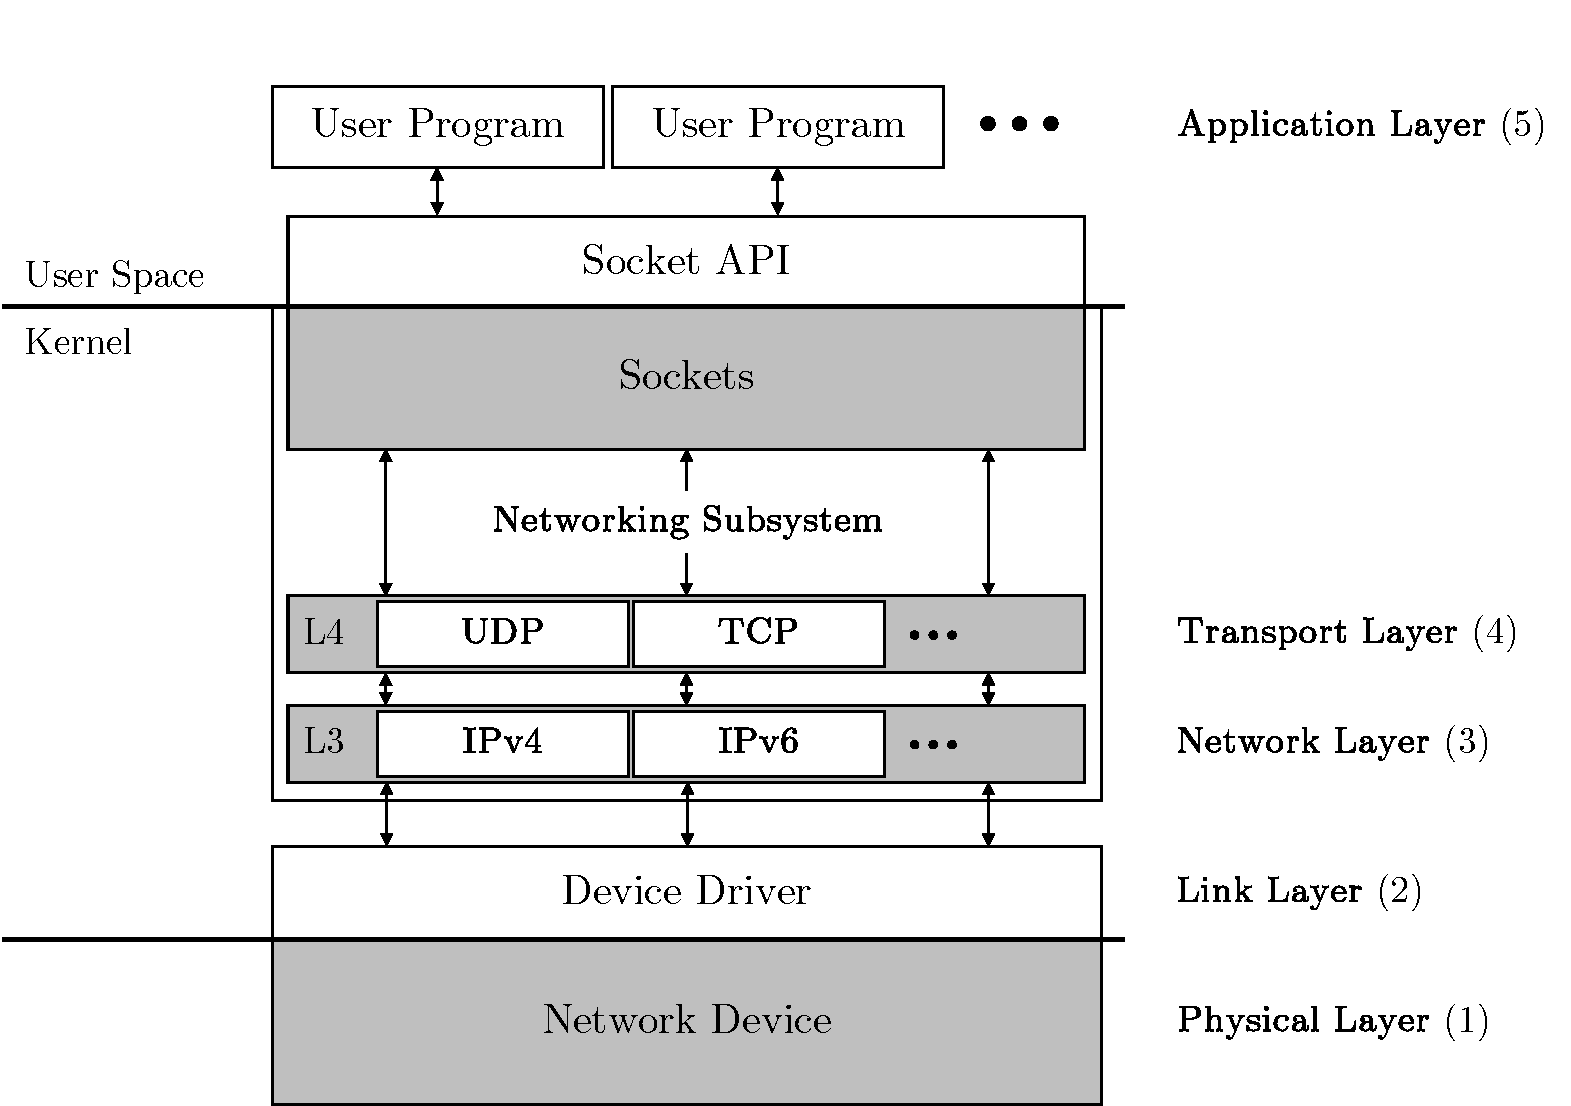
\includegraphics[width=1\linewidth]{figures/linux_nwstack/image03.pdf}
    \caption[Simplified Representation of the Linux Network Stack with associated Layers of the hybrid TCP/IP Reference Model]{Simplified Representation of the Linux Network Stack with associated Layers of the hybrid TCP/IP Reference Model. Adapted from: \cite{lins06}.}
    \label{fig:NWStack}
\end{figure}

Figure \ref{fig:NWStack} presents a simplified schematic of the components of the Linux network stack and how they relate to the layers of the hybrid TCP/IP reference model presented in Chapter \ref{chap:RefModel}. This chapter provides a simplified representation, based on \cite{lins06}, that illustrates the relationship between the components of the network stack. 

First, the components of the network stack will be presented, with a focus on the protocols represented in the TCP/IP reference model. Then, the interaction between the components will be explained by following the path of a packet through the network stack during transmission and reception.


\subsection{Components in the Linux Network Stack}

\subsubsection{Sockets and the Socket API}

Sockets are objects in the operating system that allow data to be exchanged between two applications, usually on a client-server basis. Data can also be exchanged across computer boundaries. Sockets are part of the networking subsystem in the Linux kernel. The socket \ac{api} represents the associated programming interface \cite{sock01}\cite{sock11}.

Sockets serve as the interface between the application layer and the transport layer in the Linux kernel. Sockets can be defined as the endpoints of a communication channel between two applications. They do not form a separate layer, but allow the application to access the services of the underlying layer, usually the transport layer. The operating system manages all sockets and their associated information \cite{sock02}.

\paragraph{Characteristics of Sockets}

A socket is a generic interface that supports various protocols and protocol families, also known as communication domains. This section focuses on sockets for the TCP/IP protocol family, also known as Internet sockets \cite{like03}.

\subparagraph{Socket Descriptor}
In line with the Linux philosophy of `\textit{everything is a file}', sockets in a system are also represented by an integer, called a socket descriptor in this context. This descriptor can be obtained through a specific call to the operating system and can be used to perform operations such as \texttt{write()} or \texttt{read()}, similar to handling files. Additionally, there are specialized methods like \texttt{send()} or \texttt{receive()} that provide further options.

\subparagraph{Socket Types}
There are different types of sockets that vary in their properties. The two most common types are stream sockets and datagram sockets \cite{like03}.

\begin{itemize}
\item \textbf{Stream sockets} operate in a connection-oriented manner between a client and server application. A connection must be established between the partners before data can be transferred. \ac{tcp} is used for this type for Internet sockets.
\item \textbf{Datagram sockets} enable the exchange of individual messages. The sockets operate without a connection. \ac{udp} is utilized as the transport layer protocol, resulting in the provision of unreliable transmission.
\end{itemize}

Other socket types, such as Raw sockets or Packet sockets, also exist.


\subparagraph{Socket Address}
A socket can be identified externally using the socket address. In the context of Internet sockets, this address consists of the IP address and a port number and uniquely identifies the socket globally \cite{sock02}.


\paragraph{Operation of Sockets}

The following section presents important concepts and aspects of working with sockets. The focus is limited to connectionless datagram sockets, as this is the type of socket used in this thesis. For a detailed description of datagram sockets and stream sockets, please refer to \cite{like03}, which serves as the basis for this section.

\begin{figure}[h]
    \centering
    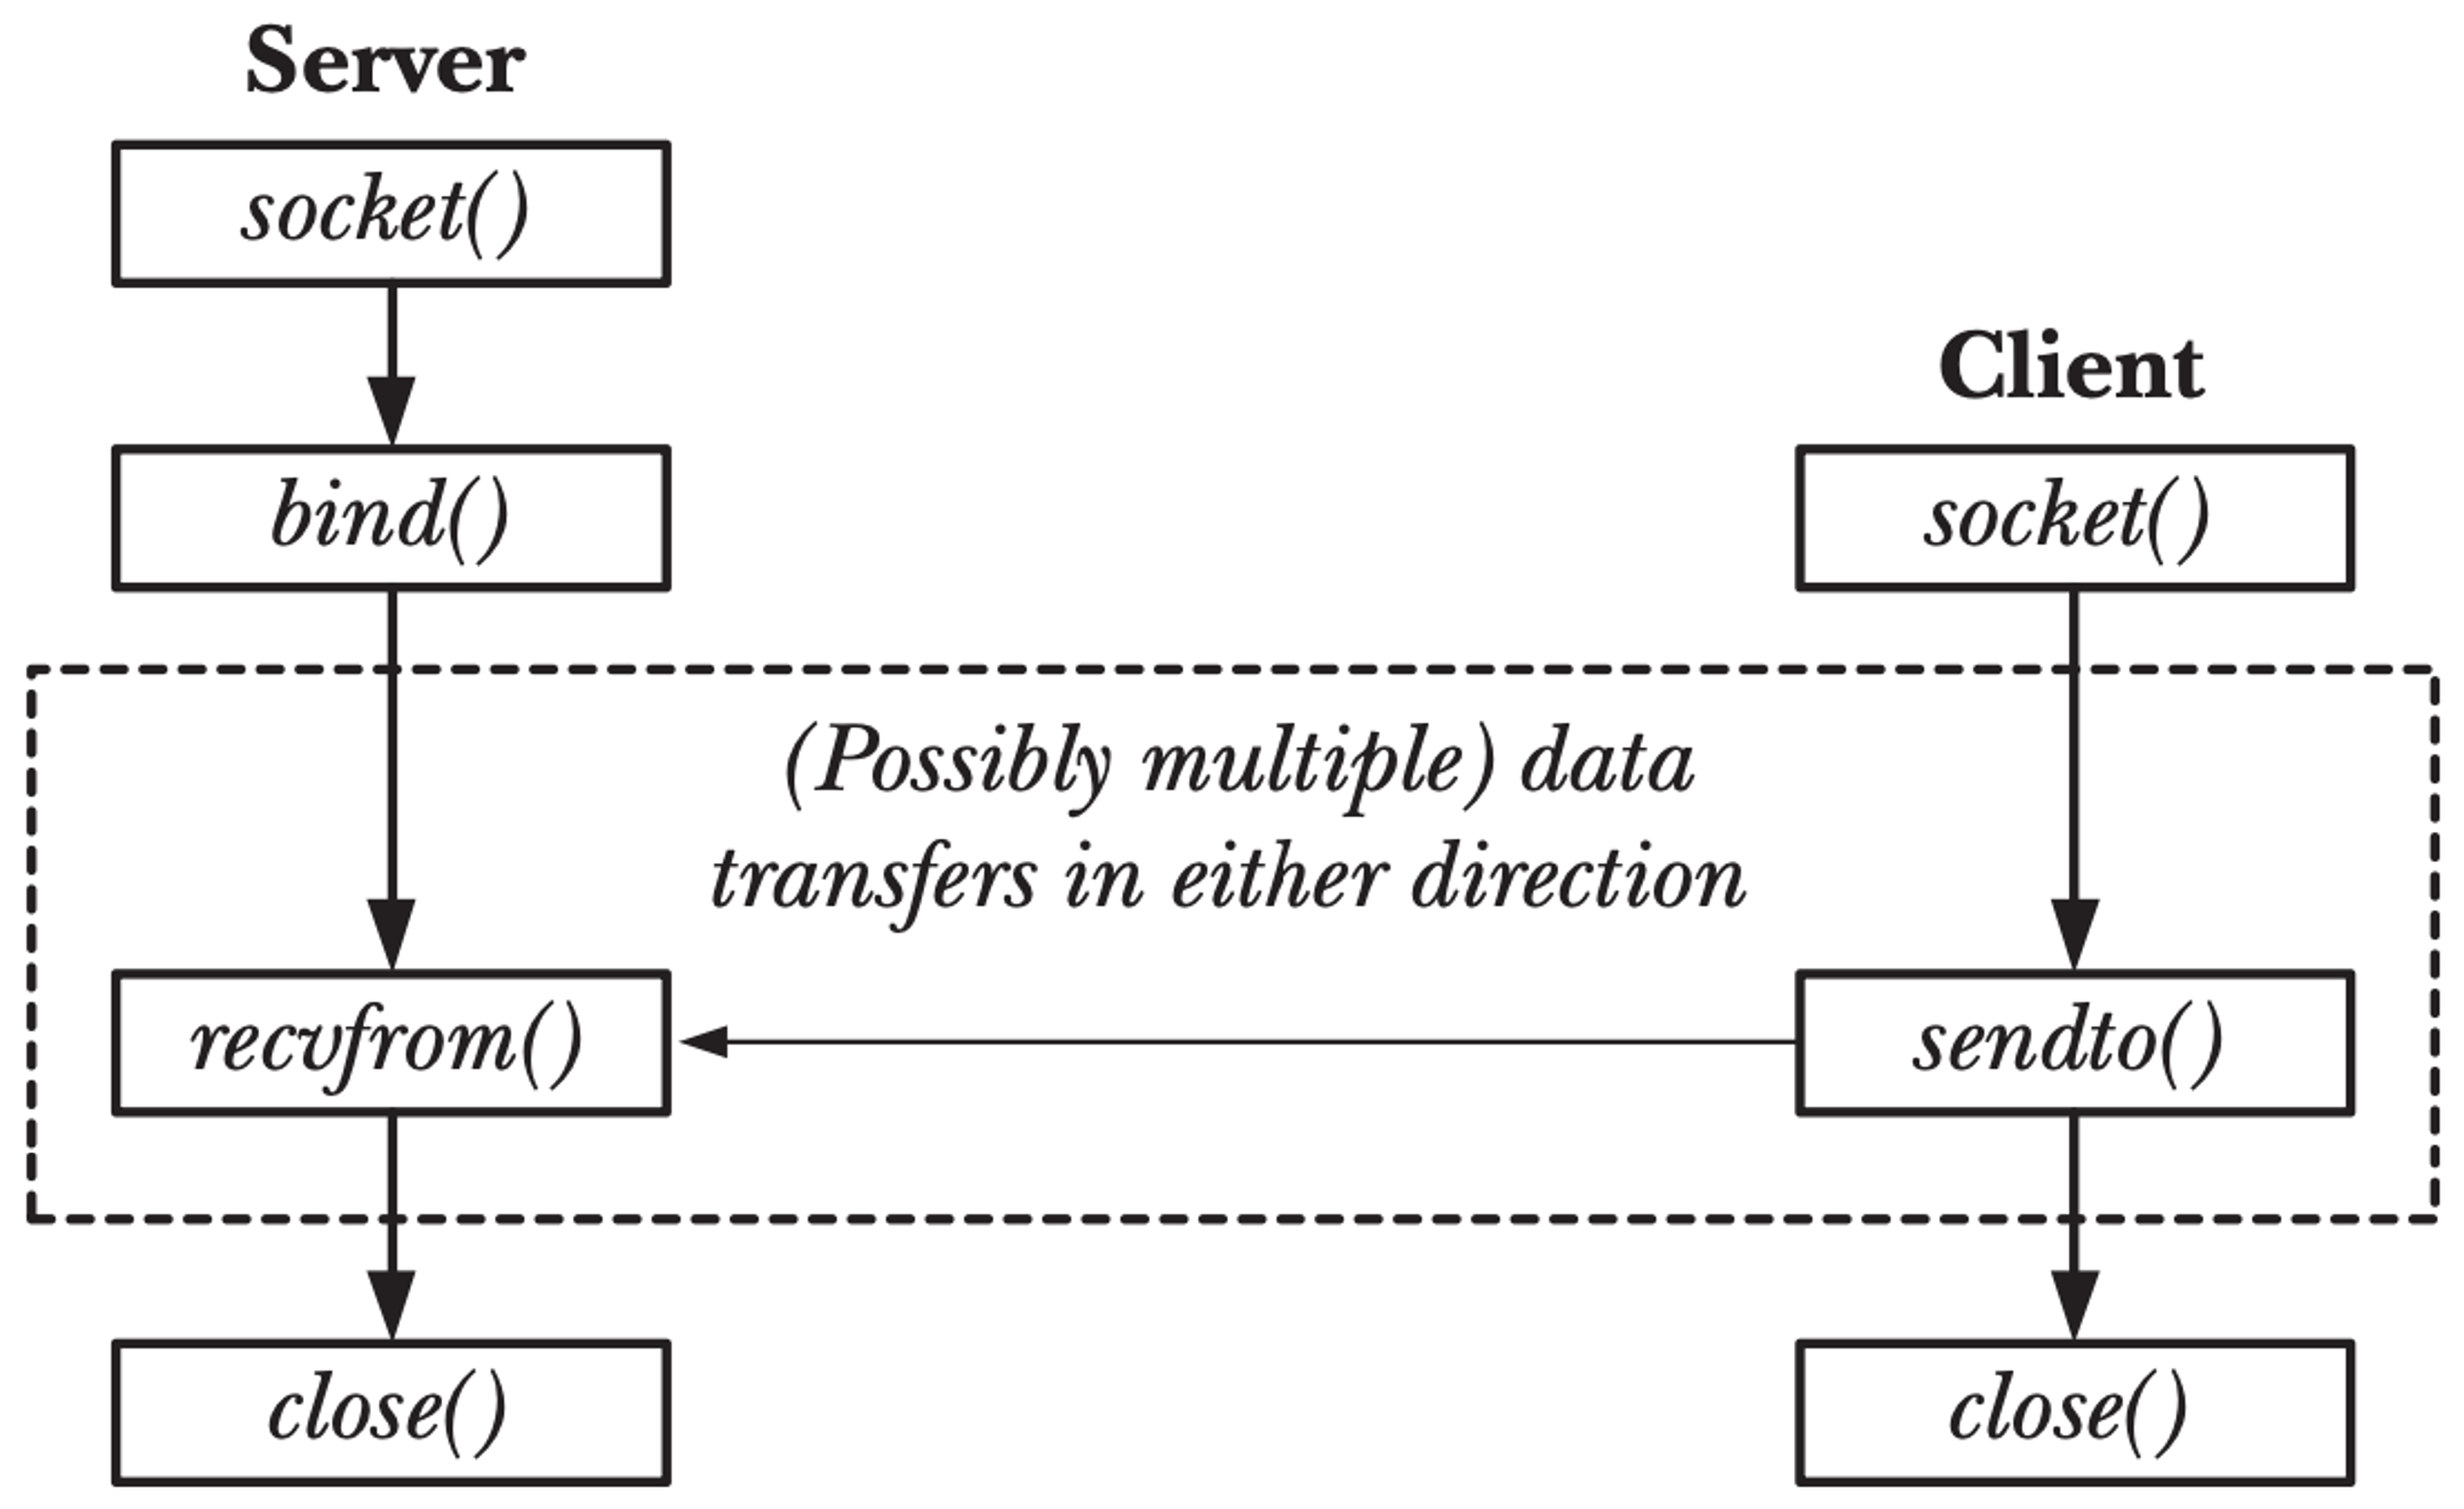
\includegraphics[width=0.75\linewidth]{figures/linux_nwstack/image01.png}
    \caption[Overview of System Calls used with Datagram Sockets]{Overview of System Calls used with Datagram Sockets. Source: \cite{like03}.}
    \label{fig:SocketOperations}
\end{figure}

Figure \ref{fig:SocketOperations} displays the system calls commonly used with a datagram socket for a client-server application. These calls are briefly described below:

\begin{itemize}
\item The \texttt{socket()} call requests the corresponding socket from the operating system, specifying the protocol family and socket type. The return value is the socket descriptor.
\item The \texttt{bind()} call is used to bind the socket to a server address. For Internet sockets, the address consists of the IP address and the port of the server application. This enables the application to receive datagrams sent to this address.
\item The client calls \texttt{sendto()} with both the data to be sent and the address of the socket to which the datagram is to be sent. This call will send the data.
\item \begin{minipage}[t]{\linewidth}
            To receive a datagram, \texttt{recvfrom()} is called. The argument can be used to specify the address of the sender's socket from which the data is to be received. If no restrictions should be defined for the sender's address, \texttt{recv()} can also be used.\\
            Both calls save exactly one received datagram in a buffer, a pointer to which is also passed as an argument to the function. If no data has been received when \texttt{recv()} or \texttt{recvfrom()} is called, the call is blocked.\\
            If multiple datagrams are received, they are stored in the receive buffer of the corresponding socket. However, when one of these functions is called, only one message is passed to the application via the socket.
      \end{minipage}
\item If the socket is no longer needed, it can be closed using \texttt{close()}.
\end{itemize}


\paragraph{Raw Sockets and Packet Sockets}

Raw sockets and Packet sockets are additional types of Internet sockets. These are an addition to the stream and datagram sockets already mentioned and allow access to lower layers of the network stack instead of hiding them from the user \cite{sock07}.

\begin{figure}[h]
    \centering
    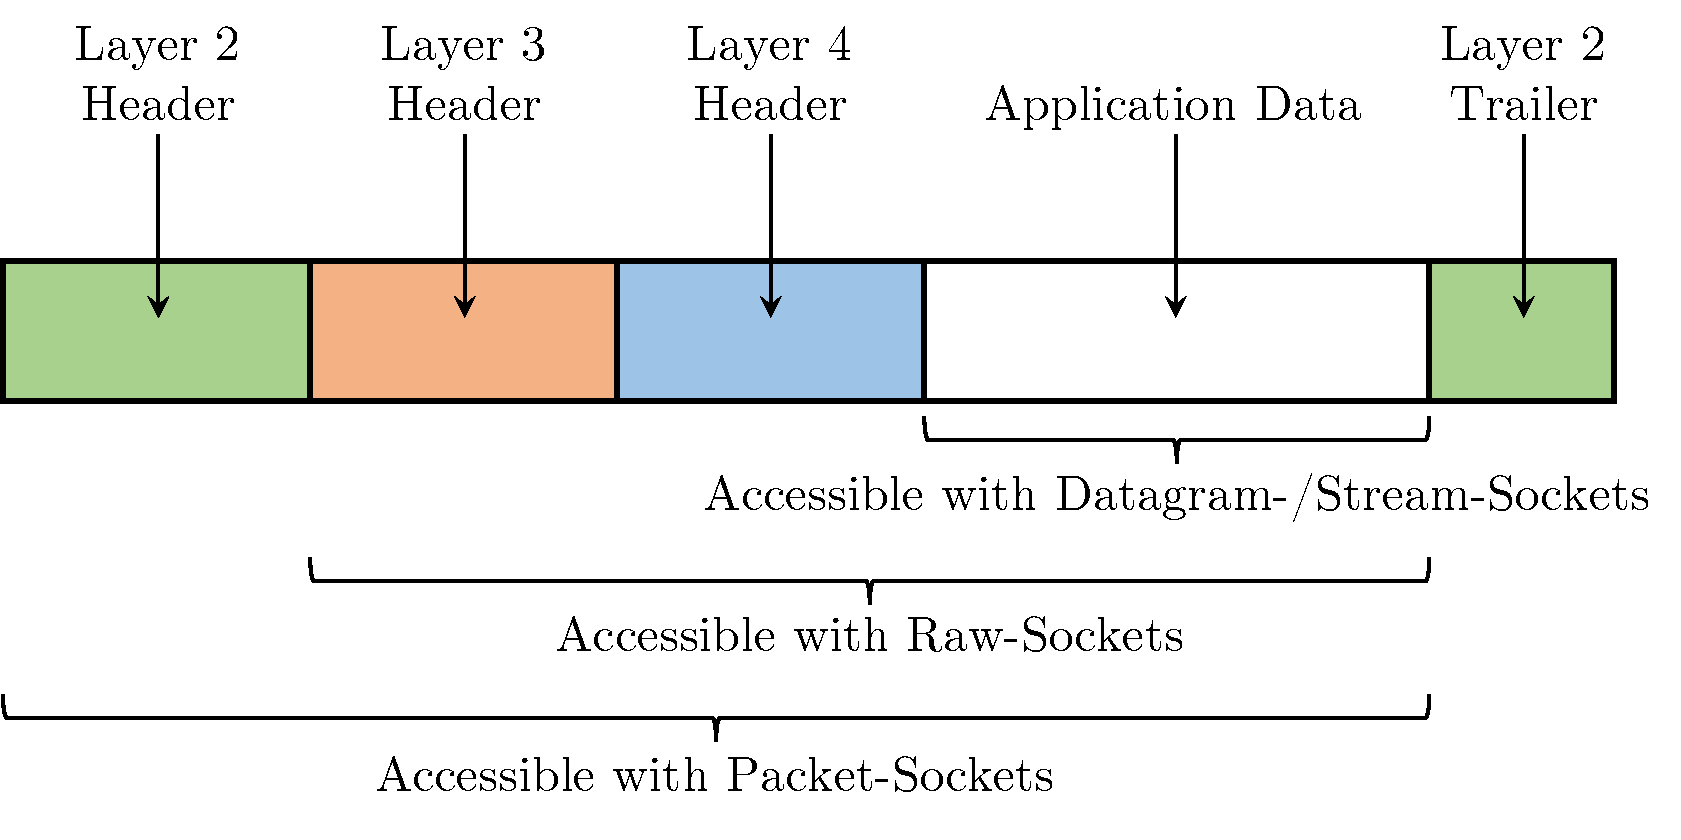
\includegraphics[width=0.9\linewidth]{figures/linux_nwstack/image02.pdf}
    \caption[Overview of Network Layers and Access Possibilities with different Socket Types]{Overview of Network Layers and Access Possibilities with different Socket Types. Adapted from: \cite{sock07}.}
    \label{fig:SocketAccessPossib}
\end{figure}

Figure \ref{fig:SocketAccessPossib} displays the access possibilities with different socket types. Raw sockets provide access to the transport layer (4) and network layer (3) of the network stack \cite{sock08}, including TCP or \ac{udp} as well as IP in the case of the TCP/IP reference model. Packet sockets in addition can also be utilized to access the link layer (2), enabling access to almost the entire Ethernet frame, except for the preamble and trailer \cite{sock09}.

The concept underlying Raw and Packet sockets involves the implementation of separate protocol layers in the application. Depending on the chosen socket type, the application can implement layers 2 to 4 \cite{sock08}. Furthermore, Packet sockets can also be used to capture the entire communication of a system, as used by Wireshark, for example.

Raw or Packet sockets eliminate the overhead of the respective protocol layer in the Linux kernel, which can potentially accelerate processing. They also increase flexibility, as certain fields in the header can be easily modified.

A disadvantage, however, is that in order to maintain compatibility with other TCP/IP implementations, the corresponding protocols must be fully and correctly implemented in the application. Additionally, using Raw or Packet sockets requires that the application be executed with root privileges.

The technical report `Introduction to RAW sockets' \cite{sock07} provides a comprehensive overview of Raw and Packet sockets and their application. This report was also used for programming in this thesis.



\subsubsection{Layers 3 and 4 in the Networking Subsystem}
The networking subsystem of the Linux kernel includes not only sockets but also layers 3 and 4, namely the transport and network layers. These layers implement the protocols described in \ref{chap:ProtosRefModel}, while sockets provide an interface between the application and the network stack.

\paragraph{Protocol Handler}
The corresponding protocols are implemented in layers 3 and 4, including implementations for protocols from the TCP/IP reference model and other protocols in their respective layers. It is also possible to develop handlers for your own protocols \cite{lins06}.

An important task in the network subsystem is to execute the correct protocol handler for the corresponding layer. For outgoing packets, this is determined by the socket. For instance, an Internet socket that uses the datagram type employs the \ac{udp} protocol at layer 4 and the IPv4 protocol at layer 3. The protocol handler to be executed for incoming packets is determined from the header of the underlying layer. Both the Ethernet header and the IP header contain a corresponding field for the service-using protocol \cite{lins06}.

The protocol handlers of the respective layer implement the standardized behavior for this protocol. These are described in the chapter \ref{chap:ProtosRefModel}. Implementation details will not be discussed further at this point. For more information, please refer to \cite{lins01}.

\paragraph{Data Structures in the Networking Subsystem of the Linux Kernel}
This chapter presents two significant data structures of the networking subsystem in the Linux kernel, as described in \cite{lins06}.

\subparagraph{Socket Buffer Structure}
The socket buffer structure, also known as \texttt{sk\_buff}, is the most important data structure in the network stack. It represents a packet that has been received or is to be sent and is used by layers 2, 3, and 4. This structure eliminates the need to copy packet data between layers.

The structure contains control information associated with a network packet, but not the actual data itself. Included in this structure are:

\begin{itemize}
\item Information on the organization of the socket buffers by the kernel
\item Pointers to the data and to the headers of layers 2, 3 and 4
\item Length of the data and the headers
\item Data on the internal coordination of the packet
\item Information on the associated network device (see \ref{chap:netdevice})
\end{itemize}

The mentioned pointers to the data point to a data field associated with the socket buffer. This field contains the packet data and associated headers and is created when a socket buffer is allocated. The socket buffer has pointers to different locations in this data field, depending on the layer currently using the socket buffer.

Additionally, there are management functions related to the socket buffers. These functions can be utilized by individual network layers to add or remove their headers to the packet during processing. There are also functions to modify the size of the data field.

\subparagraph{Network Device Structure} \label{chap:netdevice}
The network device structure, also known as \texttt{net\_device}, contains information about a specific network interface. This structure is present in the kernel for every network interface of the system.

Some important fields of this structure are (according to \cite{lins01}):
\begin{itemize}
\item Identifier of the interface
\item \ac{mtu} of the network interface
\item \ac{mac} address of the interface
\item Configurations and flags of the interface
\item Pointer to the transmit method of the interface
\end{itemize}

\subsubsection{Network Device and Device Driver}
The network device, also known as the network interface, along with its associated device driver, is the lowest component in the Linux network stack. The device driver performs the tasks of layer 2 of the TCP/IP reference model, while the network interface physically transmits the data, working on layer 1 of the reference model \cite{lins01}.

The main tasks of the device driver are to receive packets addressed to the system and forward them to layer 3 of the network stack, and to send packets generated by the system.

The driver interacts with the network interface, which transmits the data according to the respective transmission standard \cite{lins01}. To exchange data with the interface, the driver creates two ring buffers: the TX\_Ring and the RX\_Ring, which are used for sending and receiving data. These buffers are located in the system memory and contain a fixed number of descriptors pointing to buffers where packets can be stored. They are empty during initialization and accessed by the interface via \ac{dma} \cite{lins03, lins14}.

The implementation of the driver depends on the hardware and is therefore not standardized. However, the Linux kernel defines how the driver interacts with the networking subsystem.

\subsection{Path of a Network Packet} \label{chap:sedrecpath}
This section explains how a packet travels through the Linux network stack by examining the interactions of the components described above. Specifically, this section will focus on the reception and transmission of a \ac{udp} packet.

The following overview provides a general understanding of the process and will serve as a foundation. For a more detailed explanation of the packet's path, please refer to \cite{lins01} and \cite{lins06}.

\subsubsection{Receiving a Packet} \label{chap:recpath}
When a frame is received by the network card, it is first checked for errors using the Ethernet frame checksum and then verifies if it is intended for the network interface by using the \ac{mac} address. The frame is then written to a free buffer in the RX\_Ring via \ac{dma}, which was created by the device driver during initialization. If no buffers are available, the frame is dropped \cite{lins03, lins06, lins14}.

Interrupts are utilized to notify the system about a packet. Different strategies can be employed for this purpose. In the simplest case, a hardware interrupt is triggered for each received frame \cite{lins06}.

To minimize processing in the interrupt context, softirqs are utilized \cite{lins03}. Softirqs are non-urgent interruptible functions in the Linux kernel that are designed to handle tasks that do not need to be done in the interrupt context. The handlers for the softirqs are executed by ksoftirq kernel threads, with one thread for each \ac{CPU} core on the system \cite{like02}.

The network driver's hardware interrupt handler schedules a softirq to process packets for the device by adding the it to a poll list. When the corresponding softirq kernel thread is scheduled, it executes the function \texttt{net\_rx\_action} \cite{lins03}.

This function, executed in the context a softirq, processes all devices in the poll list. During the processing of the RX\_Ring of a network device, the hardware interrupts for this device are deactivated. Each  packet is wrapped in an \texttt{sk\_buff} structure and handled by an appropriate Layer 3 protocol handler. In the case of IP packets, the \texttt{ip\_rcv()} function is used. The process is repeated until there are no frames left in the RX\_Ring of the Interface or until a limit, called device weight, is reached. Additionally, a new descriptors are allocated and added to the RX\_Ring \cite{lins03, lins13, lins14}.

The \texttt{ip\_rcv()} function processes the packets as defined in the protocol, including defragmentation and routing. It then calls the appropriate protocol handler of the layer above. For \ac{udp}, this is \texttt{udp\_rcv()} \cite{lins01}.

During processing by \ac{udp}, the system verifies the availability of a socket with the corresponding port number. If available, the packet is copied into the receive buffer of the socket. If no corresponding socket is found, the packet is dropped \cite{lins01}.

Processing of the packet in the context of the softirq is now complete. The application can retrieve the packet from the receive buffer of the socket using the \texttt{receive()} call.


\subsubsection{Sending a Packet}
To send a packet, an application needs an appropriate socket, in the case of \ac{udp} packets an Internet socket of type datagram. The \texttt{sendto()} function is used to send the data, which contains the actual data as well as the address of the socket to which the data should be sent.

In the Linux kernel, calls to \texttt{sendto()} for a \ac{udp} socket are handled by the \texttt{udp\_sendmsg()} function in context of the application. This creates a socket buffer for the packet. Additionally, the \ac{udp} packet undergoes initial checks such as the compliance with the maximum length, and the \ac{udp} header is generated. Subsequently, the packet is forwarded to the IP protocol handler \cite{lins01}.

The Internet Protocol handler generates the IP header and fragments the packet if required. In addition, the protocol handler performs routing to determine which network device the packet should be sent to. This process is also performed in the context of the application \cite{lins01, lins03}.

To implement traffic management and prioritization, a layer called \ac{qdisc} is placed between the protocol handler of layer 3 and the device driver. By default, a \ac{qdisc} called 'pfifo\_fast' is used, which is essentially a \ac{fifo} queue. The queuing of the packet is also handled in the context of the application \cite{lins03, lins12}.

The actual transmission of the packet over the \ac{nic} is usually done in the context of a softirq. The device driver for the interface adds the Ethernet header and places it in the transmission queue of the interface, known as the TX\_Ring. The NIC hardware then fetches the packets from the TX\_Ring using \ac{dma} and transmits them over the physical medium. An interrupt is generated by the interface to indicate a successful transmission \cite{lins06, lins14}.


\clearpage

\section{Advanced Networking Options}

\subsection{Hardware Offloading} \label{chap:HWOffload}
Hardware offloading enables specialized hardware to perform compute-intensive tasks instead of the system's \ac{CPU}, reducing its workload. In terms of networking, this specialized hardware is integrated into the network interface \cite{tuning01}. Linux distinguishes between two types of offload: Checksum Offload and Segmentation Offload \cite{tuning02, tuning03}.

Checksum Offload refers to the ability to calculate various checksums of the protocols in the TCP/IP reference model, including the checksum in the Ethernet frame and the checksum in the IP or \ac{udp} header \cite{tuning02}.

Segmentation Offload can be used to fragment a \ac{udp} packet using the network interface. A similar technique also exists for \ac{tcp} \cite{tuning03}.


\subsection{Receive Side Scaling} \label{chap:ReceiveSideScaling}
\ac{rss} is a technology used to improve network performance. The procedure for receiving a packet is described in \ref{chap:recpath}. The interrupt and softirq described there, which carry out the processing of the received packet, are handled by a single \ac{CPU} \cite{rss01}.

The concept behind \ac{rss} is to distribute network data processing across multiple \ac{CPU} cores instead of keeping it confined to a single core. Incoming network packets are distributed to different processor cores based on a hash function \cite{rss02}.

For Intel network cards, the hash is calculated based on the packet type. The network interface parses all packet headers and uses specific fields as input values for the hash function. In the case of a non-fragmented \ac{udp} packet, the destination and source IP addresses, along with the destination and source port, are used to calculate a 32-bit hash value. This hash value determines the queue and \ac{CPU} core for processing the packet. All packets with the same input parameters are considered a related communication flow and have the same hash value. As a result, they are processed by the same \ac{CPU} \cite{rss03}.

\subsection{Interrupt Moderation} \label{chap:InterMod}
As explained in \ref{chap:sedrecpath}, the system generates an interrupt for both incoming and outgoing packets, which can negatively impact performance, particularly at high transmission rates due to the high number of interrupts generated \cite{intermod01}. Interrupt moderation can be used to mitigate this issue by delaying the generation of interrupts until multiple packets have been sent or received, or a timeout has occurred, thereby reducing \ac{CPU} utilization \cite{intermod02}.

The Intel network interface drivers enable the configuration of a fixed timeout value for interrupt moderation or the complete deactivation of interrupt moderation. By default, adaptive interrupt moderation is active, which, according to Intel, provides a balanced approach between low \ac{CPU} utilization and high performance \cite{intermod03}. The interrupt rate is dynamically set based on the number of packets, packet size, and number of connections. The associated patent \cite{intermod04} provides a detailed description of this process. Typically, the interrupt rate is set to achieve either low latency or high throughput, depending on the type of traffic. For small datagrams, a low interrupt timeout (i.e., a high number of interrupts/s) is selected, while for large datagrams, a high interrupt timeout (i.e., a lower number of interrupts/s) is selected. Additionally, the interrupt rate also depends on the number of connections, with a high interrupt rate selected for a low number of connections and a low interrupt rate selected for a high number of connections.

The interrupt moderation timeout of Intel network interfaces can be configured using the 'ethtool' configuration tool within the range of 0 to 235 µs. A value of 0 µs deactivates interrupt moderation.

\subsection{Quality of Service} \label{background:tuning:qualityofservice}
\acf{qos} comprises different mechanisms to provide distinct service levels for various network traffic. A service level includes statements about bandwidth, jitter, or reliability \cite{qos01}. To achieve a service level, \ac{qos} consists of various components and measures, including packet marking methods, traffic shaping methods, and the implementation of various queues in network devices \cite{qos02}. Due to the broad scope of \ac{qos} and its related technologies, this section only briefly introduces key technologies used.

One way to classify traffic is by using the Differentiated Services field in the IP header (refer to \ref{chap:ipheader}). This field enables the specification of a Differentiated Services Field Codepoint, which can be interpreted as a priority. The values range from 0 to 63, with 63 being the highest priority \cite{qos02}.

Differentiated Services Field Codepoints are solely used for packet classification. To achieve specific service levels in the network, it is necessary to configure the network hardware to ensure the desired traffic handling. This may involve prioritizing certain Differentiated Services Field Codepoint values over others \cite{qos02}.

